% Options for packages loaded elsewhere
\PassOptionsToPackage{unicode}{hyperref}
\PassOptionsToPackage{hyphens}{url}
%
\documentclass[
]{article}
\usepackage{lmodern}
\usepackage{amssymb,amsmath}
\usepackage{ifxetex,ifluatex}
\ifnum 0\ifxetex 1\fi\ifluatex 1\fi=0 % if pdftex
  \usepackage[T1]{fontenc}
  \usepackage[utf8]{inputenc}
  \usepackage{textcomp} % provide euro and other symbols
\else % if luatex or xetex
  \usepackage{unicode-math}
  \defaultfontfeatures{Scale=MatchLowercase}
  \defaultfontfeatures[\rmfamily]{Ligatures=TeX,Scale=1}
\fi
% Use upquote if available, for straight quotes in verbatim environments
\IfFileExists{upquote.sty}{\usepackage{upquote}}{}
\IfFileExists{microtype.sty}{% use microtype if available
  \usepackage[]{microtype}
  \UseMicrotypeSet[protrusion]{basicmath} % disable protrusion for tt fonts
}{}
\makeatletter
\@ifundefined{KOMAClassName}{% if non-KOMA class
  \IfFileExists{parskip.sty}{%
    \usepackage{parskip}
  }{% else
    \setlength{\parindent}{0pt}
    \setlength{\parskip}{6pt plus 2pt minus 1pt}}
}{% if KOMA class
  \KOMAoptions{parskip=half}}
\makeatother
\usepackage{xcolor}
\IfFileExists{xurl.sty}{\usepackage{xurl}}{} % add URL line breaks if available
\IfFileExists{bookmark.sty}{\usepackage{bookmark}}{\usepackage{hyperref}}
\hypersetup{
  pdftitle={Examen final - Otoño 2020},
  pdfauthor={Alfredo Garbuno Iñigo},
  hidelinks,
  pdfcreator={LaTeX via pandoc}}
\urlstyle{same} % disable monospaced font for URLs
\usepackage[margin=1in]{geometry}
\usepackage{color}
\usepackage{fancyvrb}
\newcommand{\VerbBar}{|}
\newcommand{\VERB}{\Verb[commandchars=\\\{\}]}
\DefineVerbatimEnvironment{Highlighting}{Verbatim}{commandchars=\\\{\}}
% Add ',fontsize=\small' for more characters per line
\usepackage{framed}
\definecolor{shadecolor}{RGB}{248,248,248}
\newenvironment{Shaded}{\begin{snugshade}}{\end{snugshade}}
\newcommand{\AlertTok}[1]{\textcolor[rgb]{0.94,0.16,0.16}{#1}}
\newcommand{\AnnotationTok}[1]{\textcolor[rgb]{0.56,0.35,0.01}{\textbf{\textit{#1}}}}
\newcommand{\AttributeTok}[1]{\textcolor[rgb]{0.77,0.63,0.00}{#1}}
\newcommand{\BaseNTok}[1]{\textcolor[rgb]{0.00,0.00,0.81}{#1}}
\newcommand{\BuiltInTok}[1]{#1}
\newcommand{\CharTok}[1]{\textcolor[rgb]{0.31,0.60,0.02}{#1}}
\newcommand{\CommentTok}[1]{\textcolor[rgb]{0.56,0.35,0.01}{\textit{#1}}}
\newcommand{\CommentVarTok}[1]{\textcolor[rgb]{0.56,0.35,0.01}{\textbf{\textit{#1}}}}
\newcommand{\ConstantTok}[1]{\textcolor[rgb]{0.00,0.00,0.00}{#1}}
\newcommand{\ControlFlowTok}[1]{\textcolor[rgb]{0.13,0.29,0.53}{\textbf{#1}}}
\newcommand{\DataTypeTok}[1]{\textcolor[rgb]{0.13,0.29,0.53}{#1}}
\newcommand{\DecValTok}[1]{\textcolor[rgb]{0.00,0.00,0.81}{#1}}
\newcommand{\DocumentationTok}[1]{\textcolor[rgb]{0.56,0.35,0.01}{\textbf{\textit{#1}}}}
\newcommand{\ErrorTok}[1]{\textcolor[rgb]{0.64,0.00,0.00}{\textbf{#1}}}
\newcommand{\ExtensionTok}[1]{#1}
\newcommand{\FloatTok}[1]{\textcolor[rgb]{0.00,0.00,0.81}{#1}}
\newcommand{\FunctionTok}[1]{\textcolor[rgb]{0.00,0.00,0.00}{#1}}
\newcommand{\ImportTok}[1]{#1}
\newcommand{\InformationTok}[1]{\textcolor[rgb]{0.56,0.35,0.01}{\textbf{\textit{#1}}}}
\newcommand{\KeywordTok}[1]{\textcolor[rgb]{0.13,0.29,0.53}{\textbf{#1}}}
\newcommand{\NormalTok}[1]{#1}
\newcommand{\OperatorTok}[1]{\textcolor[rgb]{0.81,0.36,0.00}{\textbf{#1}}}
\newcommand{\OtherTok}[1]{\textcolor[rgb]{0.56,0.35,0.01}{#1}}
\newcommand{\PreprocessorTok}[1]{\textcolor[rgb]{0.56,0.35,0.01}{\textit{#1}}}
\newcommand{\RegionMarkerTok}[1]{#1}
\newcommand{\SpecialCharTok}[1]{\textcolor[rgb]{0.00,0.00,0.00}{#1}}
\newcommand{\SpecialStringTok}[1]{\textcolor[rgb]{0.31,0.60,0.02}{#1}}
\newcommand{\StringTok}[1]{\textcolor[rgb]{0.31,0.60,0.02}{#1}}
\newcommand{\VariableTok}[1]{\textcolor[rgb]{0.00,0.00,0.00}{#1}}
\newcommand{\VerbatimStringTok}[1]{\textcolor[rgb]{0.31,0.60,0.02}{#1}}
\newcommand{\WarningTok}[1]{\textcolor[rgb]{0.56,0.35,0.01}{\textbf{\textit{#1}}}}
\usepackage{graphicx,grffile}
\makeatletter
\def\maxwidth{\ifdim\Gin@nat@width>\linewidth\linewidth\else\Gin@nat@width\fi}
\def\maxheight{\ifdim\Gin@nat@height>\textheight\textheight\else\Gin@nat@height\fi}
\makeatother
% Scale images if necessary, so that they will not overflow the page
% margins by default, and it is still possible to overwrite the defaults
% using explicit options in \includegraphics[width, height, ...]{}
\setkeys{Gin}{width=\maxwidth,height=\maxheight,keepaspectratio}
% Set default figure placement to htbp
\makeatletter
\def\fps@figure{htbp}
\makeatother
\setlength{\emergencystretch}{3em} % prevent overfull lines
\providecommand{\tightlist}{%
  \setlength{\itemsep}{0pt}\setlength{\parskip}{0pt}}
\setcounter{secnumdepth}{-\maxdimen} % remove section numbering

\title{Examen final - Otoño 2020}
\author{Alfredo Garbuno Iñigo}
\date{}

\begin{document}
\maketitle

\textbf{Entrega:} Enviar la carpeta que el codigo de solución (.Rmd y
funciones auxiliares) a mas tardar el 15 de Diciembre antes de las
12:00pm (mediodia), por correo electrónico con el título
fundamentos-final, un solo documento por equipo. No se aceptarán
entregas extemporáneas. Será mejor entregar un examen resuelto
parcialmente, que no entregar nada.

\textbf{Instrucciones:}

\begin{itemize}
\item
  Tus respuestas deben ser claras y debes explicar los resultados,
  incluye también tus procedimientos/código de manera ordenada, y el
  código comentado.
\item
  Se evaluará la presentación de resultados (calidad de las gráficas,
  tablas,\ldots), revisa la sección de visualización en las notas.
\item
  Las sesiones del Martes 8 y Jueves 10 de Diciembre a las 10 am, serán
  espacios para resolver dudas que puedan surgir del exámen.
\item
  No pueden compartir soluciones entre diferentes equipos, o alumnos del
  grupo 001 de esta misma materia.
\item
  Al entregar este examen afirmas que el trabajo se realizó sólo con tu
  compañero de equipo. El material que utilizaste para apoyarte
  consistió de las notas en clase (pdf en canvas), el codigo fuente de
  las notas en el repositorio de Github.
\item
  Al entregar estás dando tu consentimiento para que bajo sospecha y
  suficiente evidencia de copia se anule tu evaluación.
\end{itemize}

\hypertarget{preparaciuxf3n-de-ambiente}{%
\section{Preparación de ambiente}\label{preparaciuxf3n-de-ambiente}}

Asegurate de tener instalado los paquetes que usamos más en las notas
del curso. En particular, si usas \texttt{renv} como manejador de
ambientes puedes instalarlos con las instrucciones de abajo. Sólo
necesitarías descomentarlas.

\begin{Shaded}
\begin{Highlighting}[]
\CommentTok{# renv::install("tidyverse")}
\CommentTok{# renv::install("patchwork")}
\CommentTok{# renv::install("nullabor")}
\CommentTok{# renv::install("scales")}
\CommentTok{# renv::install('diegovalle/mxmaps')}
\CommentTok{# renv::install("nleqslv")}
\CommentTok{# renv::snapshot()}

\CommentTok{# Escribe las claves unicas de ambos miembros del equipo, para generar una}
\CommentTok{# semilla de numeros aleatorios.}
\NormalTok{claves_unicas <-}\StringTok{ }\KeywordTok{c}\NormalTok{(}\DecValTok{151280}\NormalTok{, }\DecValTok{150370}\NormalTok{)}
\KeywordTok{set.seed}\NormalTok{(}\KeywordTok{min}\NormalTok{(claves_unicas))}
\end{Highlighting}
\end{Shaded}

\hypertarget{modelos-de-conteo}{%
\section{Modelos de conteo}\label{modelos-de-conteo}}

En el curso hemos estudiado las variables aleatorias Gaussianas para
modelar eventos aleatorios compuestos de pequeños, pero controlados,
efectos. También hemos utilizado variables aleatorias Binomiales para
modelar tasas de éxito de algún evento binario de interés. En el
contexto Bayesiano, hemos utilizado las distribuciones Beta,
Gamma-Inversa, y Normal para realizar análisis conjugado con estos
modelos.

En este mini-proyecto, ilustraremos otra familia de distribuciones muy
cómunes en la práctica. En particular, veremos la distribución
\textbf{Poisson} como unmodelo de conteo. Es decir, una variable
aleatoria Poisson nos sirve para modelar el número de ocurrencias de un
evento en un periodo (tiempo) o área (espacio) base.

Decimos que \(x|\theta \sim \textsf{Poisson}(\theta)\) si los eventos
ocurren de manera independiente y a una tasa constante. La función de
masa de probabilidad esta dada por

\[ p(X = k \, | \, \theta) = \frac{\theta^k \, e^{-\theta}}{k!},\]

donde sabemos que

\[ \mathbb{E}[x|\theta] = \theta, \qquad  \mathbb{V}[x|\theta] = \theta \]

Al examinar la base de la función de masa de probabilidad notamos que un
candidato para un anålisis conjugado es una distribución Gamma. Es
decir, un candidato \emph{natural} para una distribución previa para
\(\theta\) es

\[\theta \sim \textsf{Gamma}(\alpha, \beta),\]

donde la densidad está dada por

\[ p(\theta) \propto \theta^{\alpha - 1} \, e^{-\beta \, \theta},\]

y tenemos los siguientes momentos

\[\mathbb{E}[\theta] = \frac\alpha\beta, \qquad  \mathbb{V}[\theta] = \frac{\alpha}{\beta^2}.\]

\begin{center}\rule{0.5\linewidth}{0.5pt}\end{center}

\textbf{Pregunta 1)} Para una muestra
\(X_1, \ldots, X_n \overset{iid}{\sim} \textsf{Poisson}(\theta),\)
determina la distribución posterior de \(\theta,\) y calcula media y
varianza de la distribución posterior. ¿Podríamos escribir la media
posterior como un promedio ponderado entre datos e información previa?
¿Cómo interpretas los hiper-parámetros \((\alpha, \beta)?\)

\[
\begin{align}
\Pi (\theta \mid x_1 , \dots, x_n) 
&\propto \Pi (x_1, \dots, x_n \mid \theta) \cdot \Pi (\theta) \\
&\propto \prod_i{\Pi(x_i \mid \theta)} \cdot \Pi(\theta) \\
&\propto \prod_i{\frac{\theta^{x_i} e^{-\theta}}{x_i!}} \cdot \theta^{\alpha-1}e^{-\beta \theta} \\
&\propto \frac{\theta^{\sum{x_i}}e^{-n\theta}}{\prod{x_i!}} \cdot \theta^{\alpha-1}e^{-\beta \theta} \\
&\propto \theta^{\alpha + \sum{x_i} - 1}e^{-\theta(\beta + n)}
\end{align}
\] De lo anterior se puede ver que

\[
\Pi (\theta \mid x_1 , \dots, x_n)\sim Gamma(\alpha + \sum{x_i}, \beta + n)
\] Así,

\[
E[\theta \mid x_1 , \dots, x_n] = \frac{\alpha + \sum{x_i}}{\beta + n} \\
Var[\theta \mid x_1 , \dots, x_n] = \frac{\alpha + \sum{x_i}}{(\beta + n)^2} 
\] Sí se puede ver como un promedio entre los datos y el parámetro
\(\alpha\). Entre más datos sean más peso tendrán en la posterior. En
cambio si los datos \(n \to 0\), la posterior será igual a la
distribución a priori.

\begin{center}\rule{0.5\linewidth}{0.5pt}\end{center}

Otra variable aleatoria de conteo relevante es la \textbf{Binomial
Negativa.} Esta distribución sirve para modelar el número de éxitos en
una secuencia de experimentos Bernoulli antes de encontrar un número
específico de fracasos.

Decimos que \(X|\alpha, \beta \sim \textsf{Neg-Bin}(\alpha, \beta),\)
donde \(X\) es el número de éxitos que contamos antes de \(\alpha\)
fracasos, cuando cada fracaso ocurre con probabilidad
\(\frac{\beta}{\beta + 1}.\) La función de masa de probabilidad se
escribe

\[ p(X = k \, | \, \alpha, \beta) = {\alpha + k -1 \choose k} \left(\frac{\beta}{\beta + 1}\right)^\alpha \left(\frac{1}{\beta + 1}\right)^k.\]

Nota que
\[{\alpha + k -1 \choose k} = {\alpha + k -1 \choose \alpha -1},\] es
decir, el número de formas que puedes acomodar \(\alpha - 1\) fracasos
es igual al número de formas que puedes acomodar \(k\) éxitos cuando
realizaste \(\alpha + k-1\) experimentos y todos los experimentos son
independientes. Por otro lado, la definición es
\[{\alpha + k -1 \choose k} = \frac{(\alpha + k - 1)!}{k! \, (\alpha - 1)!}.\]
donde \(k! = k \times k-1 \times k-2 \times \cdots \times 1,\) y la
función Gamma satisface \[\Gamma(\alpha) = (\alpha - 1)!.\]

\begin{center}\rule{0.5\linewidth}{0.5pt}\end{center}

\textbf{Pregunta 2)} Bajo el modelo conjugado que escribiste en la
pregunta 1, calcula la \textbf{distribución predictiva previa} para una
observación Poisson. Es decir, calcula
\[p(y) = \int \textsf{Poisson}(y \,| \,\theta) \textsf{Gamma}(\theta \, | \, \alpha, \beta) \, \text{d}\theta.\]

\[
\begin{align}
p(y) &= \int_0^{\infty} \frac{\theta^y e^{-\theta}}{y!} \cdot
\frac{\beta^\alpha \theta^{\alpha-1} e^{-\beta \theta}}{\Gamma(\alpha)} d\theta \\
&= \frac{\beta^\alpha}{\Gamma(\alpha)y!} 
\int_0^\infty\theta^{y+\alpha -1}e^{-\theta(\beta +1)}d\theta
\end{align}
\] Sabemos que: \[ \Gamma(z) = \int_0^\infty t^{z-1}e^{-t}dt\] Entonces
si:

\[
t = \theta(\beta +1)\\
\Rightarrow \theta = \frac{t}{\beta +1} \\
d\theta = \frac{1}{\beta +1}dt
\] Así: \[
\begin{align}
&= \frac{\beta^\alpha}{\Gamma(\alpha)y!} 
\int_0^\infty\frac{t}{\beta +1}^{y+\alpha -1}e^{-t} \frac{1}{\beta +1}dt \\
&= \frac{\beta^\alpha}{\Gamma(\alpha)y!}\cdot\frac{1}{(\beta+1)^{y+\alpha}} \int_0^\infty t^{y+\alpha -1}e^{-t}dt \\
&= \frac{\beta^\alpha}{\Gamma(\alpha)y!}\cdot\frac{1}{(\beta+1)^{y+\alpha}} \Gamma(y+\alpha) \\
&= \frac{\Gamma(y+\alpha)}{\Gamma(\alpha)y!}  \frac{\beta^\alpha}{(\beta+1)^{y+\alpha}} \\
&=\frac{(y+\alpha-1)!}{(\alpha-1)!y!} \left(\frac{\beta}{\beta+1}\right)^\alpha \left(\frac{1}{\beta+1}\right)^y \\
&=\binom{y+\alpha-1}{y} \left(\frac{\beta}{\beta+1}\right)^\alpha \left(\frac{1}{\beta+1}\right)^y
\end{align}
\]

Verifica tu cálculo utilizando las reglas probabilidad condicional. En
especifico, utiliza

\[ p(y) = \frac{p(y|\theta)p(\theta)}{p(\theta|y)}.\] Tenemos que:

\[
\begin{align}
p(y) &= \frac{ \frac{\theta^y e^{-\theta}}{y!} \frac{\beta^\alpha\theta^{\alpha-1}e^{-\beta\theta}}{\Gamma(\alpha)}}
{\frac{(\beta+1)^{\alpha+y}\theta^{\alpha+y-1}e^{-(\beta+1)\theta}}{\Gamma(\alpha+y)}} \\
&= \frac{\Gamma(\alpha+y)}{\Gamma(\alpha)y!} \frac{\beta^\alpha}{(\beta+1)^{\alpha + y}}\theta^0e^0 \\
&=\frac{(y+\alpha-1)!}{(\alpha-1)!y!} \left(\frac{\beta}{\beta+1}\right)^\alpha \left(\frac{1}{\beta+1}\right)^y \\
&=\binom{y+\alpha-1}{y} \left(\frac{\beta}{\beta+1}\right)^\alpha \left(\frac{1}{\beta+1}\right)^y
\end{align}
\] ¿Qué distribución marginal tiene \(y\) bajo el modelo conjugado?

Es una distrubución binomial negativa, por lo tanto
\[ p(y) \sim BinNeg(\alpha,\beta)\]

\begin{center}\rule{0.5\linewidth}{0.5pt}\end{center}

En la práctica, es útil extender el modelo Poisson como sigue
\begin{align}
  x_i | t_i, \theta &\sim \textsf{Poisson}(\lambda_i), \\
  \lambda_i &= t_i \theta, 
\end{align}

donde la tasa de ocurrencia \(\lambda_i\) ha sido descompuesta en un
producto que incorpora la exposición \(t_i\) y una tasa de ocurrencia
por unidades expuestas \(\theta.\) En este contexto usualmente tenemos
observaciones para \(x_i\) y \(t_i\) pues conocemos el parámetro de
exposición. Por ejemplo, si \(x_i\) es el número de personas que se
enferman de gripe en la \(i\)-ésima ciudad en un año, entonces
\(\theta\) denota la tasa anual por persona de enfermarse de gripe en
una población de tamaño \(t_i\).

\textbf{Pregunta 3)} Supongamos que tenemos datos
\(X_1, \ldots, X_n \sim \textsf{Poisson}(\lambda_i),\) con
\(\lambda_i = t_i \theta\) para \(i = 1, \ldots, n.\) Utilizando el
modelo conjugado, ¿cuál es la distribución posterior de \(\theta?\)

\[
\begin{align}
\Pi (\theta \mid x_1 , \dots, x_n) 
&\propto \Pi (x_1, \dots, x_n \mid \theta) \cdot \Pi (\theta) \\
&\propto \prod_i{\Pi(x_i \mid \theta)} \cdot \Pi(\theta) \\
&\propto \prod_i{\frac{(\theta t_i)^{x_i} e^{-\theta t_i}}{x_i!}} \cdot \theta^{\alpha-1}e^{-\beta \theta} \\
&\propto \theta^{\sum{x_i}}e^{-\theta\sum t_i} \cdot \theta^{\alpha-1}e^{-\beta \theta} \\
&\propto \theta^{\alpha + \sum{x_i} - 1}e^{-\theta(\beta + \sum t_i)}
\end{align}
\]

Por lo tanto, la distribución posterior es: \[
\Pi (\theta\mid x_1 ,\dots,x_n)\sim Gamma(\alpha + \sum{x_i}, \beta + \sum t_i)
\]

\begin{center}\rule{0.5\linewidth}{0.5pt}\end{center}

\hypertarget{caso-de-estudio-tasas-de-mortalidad}{%
\section{Caso de estudio: Tasas de
mortalidad}\label{caso-de-estudio-tasas-de-mortalidad}}

El INEGI publica para cada año los registros de fallecimiento junto con
la causa principal de muerte. En esta sección utilizaremos los modelos
descritos anteriormente para inferir tasa de fallecimiento por Neumonía
para cada uno de los municipios/delegaciones del país. Contamos con los
últimos 5 años de los registros de defunción.

\begin{center}\rule{0.5\linewidth}{0.5pt}\end{center}

\hypertarget{carga-y-preparaciuxf3n-de-datos}{%
\subsubsection{Carga y preparación de
datos}\label{carga-y-preparaciuxf3n-de-datos}}

\textbf{Pregunta 4)} Empecemos explorando los datos. Carga los datos
para un año que elijas. Encontrarás en los archivos en
\texttt{datos/poblacion/defunciones/\textless{}año\textgreater{}} los
registros de defunciones por Neumonía para el
\texttt{\textless{}año\textgreater{}} que escojas.

\begin{Shaded}
\begin{Highlighting}[]
\NormalTok{defunciones <-}\StringTok{ }\KeywordTok{read_csv}\NormalTok{(}\StringTok{"./datos_examen/poblacion/defunciones/2019/defunciones_registradas.csv"}\NormalTok{)}


\KeywordTok{str}\NormalTok{(defunciones)}
\end{Highlighting}
\end{Shaded}

\begin{verbatim}
## tibble [30,327 x 5] (S3: spec_tbl_df/tbl_df/tbl/data.frame)
##  $ entidad    : chr [1:30327] "01" "01" "01" "01" ...
##  $ municipio  : chr [1:30327] "001" "001" "001" "003" ...
##  $ sexo       : chr [1:30327] "mujer" "hombre" "mujer" "mujer" ...
##  $ edad       : num [1:30327] 55 81 82 83 82 55 0 66 76 75 ...
##  $ edad_grupos: chr [1:30327] "[25,64)" "[64,Inf]" "[64,Inf]" "[64,Inf]" ...
##  - attr(*, "spec")=
##   .. cols(
##   ..   entidad = col_character(),
##   ..   municipio = col_character(),
##   ..   sexo = col_character(),
##   ..   edad = col_double(),
##   ..   edad_grupos = col_character()
##   .. )
\end{verbatim}

\begin{Shaded}
\begin{Highlighting}[]
\KeywordTok{map_int}\NormalTok{(defunciones[,}\DecValTok{1}\OperatorTok{:}\DecValTok{5}\NormalTok{], }\OperatorTok{~}\KeywordTok{length}\NormalTok{(}\KeywordTok{unique}\NormalTok{(.x)) )}
\end{Highlighting}
\end{Shaded}

\begin{verbatim}
##     entidad   municipio        sexo        edad edad_grupos 
##          33         314           3         114           7
\end{verbatim}

\begin{itemize}
\item
  El dataset contiene \(5\) variables y tenemos un total de \(30,327\)
  observaciones.
\item
  Observemos que tenemos \(33\) entidades, lo cual hace un poco de
  ruido, ya que, la República Mexicana está constituída por \(32\)
  entidades federativas.
\item
  En el dataset se tiene información de \(314\) municipios, de acuerdo a
  informaicón declarada por el
  \href{http://cuentame.inegi.org.mx/territorio/division/default.aspx?tema=T\#:~:text=Para\%20gobernar\%2C\%20organizar\%20y\%20administrar,todo\%20el\%20pa\%C3\%ADs\%202\%20457.}{INEGI}
  hay un total de \(2,465\) municipios, por lo que nuestra muestra
  contiene aproximadamente el \(12\%\) de ellos.
\item
  Para el sexo aparecen \(3\) categorías (intuitivamente diríamos que es
  Masculino, Femenino y No declarado).
\item
  Tenemos \(7\) grupos de edad, los cuales son los siguientes:
\end{itemize}

\begin{Shaded}
\begin{Highlighting}[]
\NormalTok{defunciones}\OperatorTok{$}\NormalTok{edad_grupos }\OperatorTok\StringTok{ }\NormalTok{unique}
\end{Highlighting}
\end{Shaded}

\begin{verbatim}
## [1] "[25,64)"  "[64,Inf]" "[0,3)"    "[3,6)"    "[6,12)"   "[18,25)"  "[12,18)"
\end{verbatim}

\begin{itemize}
\tightlist
\item
  \([3, 6)\)
\item
  \([6, 12)\)
\item
  \([12, 18)\)
\item
  \([18, 25)\)
\item
  \([25, 64)\)
\item
  \([64, \inf)\)
\end{itemize}

Para el tema de los \(33\) estados analicemos los valores:

\begin{Shaded}
\begin{Highlighting}[]
\NormalTok{defunciones}\OperatorTok{$}\NormalTok{entidad }\OperatorTok\StringTok{ }\KeywordTok{unique}\NormalTok{() }\OperatorTok\StringTok{ }\KeywordTok{sort}\NormalTok{()}
\end{Highlighting}
\end{Shaded}

\begin{verbatim}
##  [1] "01" "02" "03" "04" "05" "06" "07" "08" "09" "10" "11" "12" "13" "14" "15"
## [16] "16" "17" "18" "19" "20" "21" "22" "23" "24" "25" "26" "27" "28" "29" "30"
## [31] "31" "32" "99"
\end{verbatim}

Nótese que se tiene una entidad \(99\), que por intuición indicaríamos
que es una Entidad no identificada.

Y ahora para la variable sexo:

\begin{Shaded}
\begin{Highlighting}[]
\NormalTok{defunciones}\OperatorTok{$}\NormalTok{sexo }\OperatorTok\StringTok{ }\KeywordTok{unique}\NormalTok{() }\OperatorTok\StringTok{ }\KeywordTok{sort}\NormalTok{()}
\end{Highlighting}
\end{Shaded}

\begin{verbatim}
## [1] "hombre" "mujer"  "NaN"
\end{verbatim}

Nuestra hipótesis era casi correcta, tenemos un tercer sexo el cual es
NaN, que indica nos sugiere que el usuario no se identificó con alguno
de los 2 sexos o bien, no quiso declarar esa información.

Ahora analicemos un poco la variabilidad de los datos.

\begin{Shaded}
\begin{Highlighting}[]
\NormalTok{defunciones }\OperatorTok\StringTok{ }
\StringTok{  }\KeywordTok{ggplot}\NormalTok{(}\DataTypeTok{data =}\NormalTok{ ., }\KeywordTok{aes}\NormalTok{(}\DataTypeTok{x =}\NormalTok{ edad)) }\OperatorTok{+}
\StringTok{  }\KeywordTok{geom_boxplot}\NormalTok{(}\KeywordTok{aes}\NormalTok{(}\DataTypeTok{color =}\NormalTok{ sexo)) }\OperatorTok{+}
\StringTok{  }\KeywordTok{ggtitle}\NormalTok{(}\StringTok{'Edad por sexo declarado'}\NormalTok{) }\OperatorTok{+}
\StringTok{  }\KeywordTok{xlab}\NormalTok{(}\StringTok{'Edad'}\NormalTok{) }\OperatorTok{+}
\StringTok{  }\KeywordTok{ylab}\NormalTok{(}\StringTok{'Frecuencia relativa'}\NormalTok{) }\OperatorTok{+}
\StringTok{  }\NormalTok{ggthemes}\OperatorTok{::}\KeywordTok{theme_base}\NormalTok{()}
\end{Highlighting}
\end{Shaded}

\begin{center}\includegraphics[width=0.99\linewidth]{examen-final-alumos-entrega_files/figure-latex/grafica defunciones por año-1} \end{center}

\begin{Shaded}
\begin{Highlighting}[]
\NormalTok{defunciones }\OperatorTok\StringTok{ }\KeywordTok{colnames}\NormalTok{()}
\end{Highlighting}
\end{Shaded}

\begin{verbatim}
## [1] "entidad"     "municipio"   "sexo"        "edad"        "edad_grupos"
\end{verbatim}

Es difícil analizar la dispersión de las edades por sexo debido a la
existencia de \(2\) valores atípicos, los cuales equivalen a la edad
\(1000\) años, lo cual no hace sentido, pues no existe ningún registro
de una persona en la historia de la humanidad que haya sobrevivido a
\(1,000\) años. Suponemos que para dichas observaciones el individuo no
quiso declarar su edad o bien hubo un error en el registro de la captura
del dato. A continuación analizaremos las edades sin dichos valores.

\begin{Shaded}
\begin{Highlighting}[]
\NormalTok{defunciones }\OperatorTok\StringTok{ }
\StringTok{  }\KeywordTok{filter}\NormalTok{(edad }\OperatorTok{<}\StringTok{ }\DecValTok{250}\NormalTok{) }\OperatorTok\StringTok{ }
\StringTok{  }\KeywordTok{ggplot}\NormalTok{(}\DataTypeTok{data =}\NormalTok{ ., }\KeywordTok{aes}\NormalTok{(}\DataTypeTok{x =}\NormalTok{ edad)) }\OperatorTok{+}
\StringTok{  }\KeywordTok{geom_boxplot}\NormalTok{(}\KeywordTok{aes}\NormalTok{(}\DataTypeTok{color =}\NormalTok{ sexo)) }\OperatorTok{+}
\StringTok{  }\KeywordTok{ggtitle}\NormalTok{(}\StringTok{'Edad filtrada por sexo declarado'}\NormalTok{) }\OperatorTok{+}
\StringTok{  }\KeywordTok{xlab}\NormalTok{(}\StringTok{'Edad'}\NormalTok{) }\OperatorTok{+}
\StringTok{  }\KeywordTok{ylab}\NormalTok{(}\StringTok{'Frecuencia relativa'}\NormalTok{) }\OperatorTok{+}
\StringTok{  }\NormalTok{ggthemes}\OperatorTok{::}\KeywordTok{theme_base}\NormalTok{()}
\end{Highlighting}
\end{Shaded}

\begin{center}\includegraphics[width=0.99\linewidth]{examen-final-alumos-entrega_files/figure-latex/defunciones sin atipicos-1} \end{center}

Realizando el filtro correspondiente es un poco más ``sencillo'' (es una
palabra que no nos gusta utilizar, ya que es relativo a la persona)
analizar la dispersión de la edad para las personas: * La mediana de
edad para mujeres es mayor que para los hombres, sin embargo, ambas
distribuciones son muy similares. * Para el sexo no declarado la edad
únicamente es 0, por lo que, para dichas observaciones el individuo no
quiso declarar su sexo ni edad.

En relación a la variable \texttt{entidad}, estos son nuestros
comentarios:

\begin{Shaded}
\begin{Highlighting}[]
\NormalTok{defunciones }\OperatorTok\StringTok{ }
\StringTok{  }\KeywordTok{select}\NormalTok{(entidad) }\OperatorTok\StringTok{ }
\StringTok{  }\KeywordTok{table}\NormalTok{() }\OperatorTok\StringTok{ }
\StringTok{  }\KeywordTok{sort}\NormalTok{(}\DataTypeTok{decreasing =} \OtherTok{TRUE}\NormalTok{)}
\end{Highlighting}
\end{Shaded}

\begin{verbatim}
## .
##   09   14   15   19   30   21   11   08   07   26   16   02   05   28   25   31 
## 4062 3427 3179 2062 1582 1378 1255 1173 1073  932  856  823  699  683  677  659 
##   20   24   17   22   12   13   10   27   32   01   18   23   06   29   99   04 
##  653  618  492  480  414  404  385  359  359  311  263  231  213  196  158  137 
##   03 
##  134
\end{verbatim}

Es difícil saber qué Estado representa cada número, ya que, no se cuenta
con un diccionario de datos. Por ahora solamente se puede indicar que el
estado \(9\), es el que tiene un mayor peso en el dataset.

\textbf{Pregunta 5)} De igual forma, carga los datos de población que
encontrarás en \texttt{datos\_examen/poblacion/demograficos}. Por el
momento, no necesitamos los grupos de edad (aunque despúes los
utilizaremos). Por ahora escribe el codigo necesario para calcular el
tamaño de la población en cada uno de los municipios.

\begin{Shaded}
\begin{Highlighting}[]
\NormalTok{poblacion <-}\StringTok{ }\KeywordTok{read_csv}\NormalTok{(}\StringTok{"./datos_examen/poblacion/demograficos/poblacion_municipios_edad.csv"}\NormalTok{)}

\NormalTok{poblacion <-}\StringTok{ }\NormalTok{poblacion }\OperatorTok\StringTok{ }
\StringTok{  }\KeywordTok{mutate}\NormalTok{(}\DataTypeTok{pob_tot =}\NormalTok{ p_0a2}\OperatorTok{+}\NormalTok{p_3a5}\OperatorTok{+}\NormalTok{p_6a11}\OperatorTok{+}\NormalTok{p_12a17}\OperatorTok{+}\NormalTok{p_18a24}\OperatorTok{+}\NormalTok{p_25a64}\OperatorTok{+}\NormalTok{pob65_mas)}
\end{Highlighting}
\end{Shaded}

\textbf{Pregunta 6)} Ahora necesitamos \emph{cruzar} las tablas de
defunciones y población para crear una tabla con ambos registros. Para
esto necesitarás la función \texttt{dplyr::full\_join}.

\begin{Shaded}
\begin{Highlighting}[]
\CommentTok{# Primero se agrupan los datos de defunciones por municipio}
\NormalTok{defunciones_mun <-}\StringTok{ }\NormalTok{defunciones }\OperatorTok\StringTok{ }
\StringTok{  }\KeywordTok{group_by}\NormalTok{(entidad, municipio) }\OperatorTok\StringTok{ }
\StringTok{  }\KeywordTok{count}\NormalTok{(}\DataTypeTok{name =} \StringTok{'defunciones'}\NormalTok{)}

\NormalTok{datos =}\StringTok{ }\NormalTok{poblacion }\OperatorTok\StringTok{ }
\StringTok{  }\KeywordTok{left_join}\NormalTok{(defunciones_mun, }\DataTypeTok{by=}\KeywordTok{c}\NormalTok{(}\StringTok{'entidad'}\NormalTok{, }\StringTok{'municipio'}\NormalTok{))}
\end{Highlighting}
\end{Shaded}

\textbf{Pregunta 7)} Con esto tendrás conocimiento de cómo cargar la
información relevante (número de defunciones y población total en cada
municipio). Sin embargo, tenemos información para las defunciones de los
últimos 5 años. Carga la información que encontrarás en
\texttt{/defunciones/} y agrupa de tal forma que tengas una tabla como
la anterior. \textbf{Importante: } Para fines de este proyecto no
necesitamos los conteos por año, sólo el agrupado. Es decir, el número
de defunciones totales de los 5 años por municipio.

\begin{Shaded}
\begin{Highlighting}[]
\CommentTok{# En la funcion cargar_defunciones, en caso de error}
\CommentTok{# Por favor escribir como parámetro la dirección donde se entuentran }
\CommentTok{# los archivos de defunciones (ej: "./datos_examen/poblacion/defunciones/")}
\NormalTok{cargar_defunciones <-}\StringTok{ }\ControlFlowTok{function}\NormalTok{(}\DataTypeTok{path=}\StringTok{"./datos_examen/poblacion/defunciones/"}\NormalTok{)\{}
\NormalTok{  x <-}\StringTok{ }\KeywordTok{list.files}\NormalTok{(path, }\DataTypeTok{full.names=}\OtherTok{TRUE}\NormalTok{, }\DataTypeTok{recursive =} \OtherTok{TRUE}\NormalTok{)}
\NormalTok{  def_acum <-}\StringTok{ }\OtherTok{NULL}
  \ControlFlowTok{for}\NormalTok{ (file }\ControlFlowTok{in}\NormalTok{ x)\{}
\NormalTok{    def <-}\StringTok{ }\KeywordTok{read_csv}\NormalTok{(file)}
\NormalTok{    def_acum <-}\StringTok{ }\NormalTok{def_acum }\OperatorTok\StringTok{ }\KeywordTok{bind_rows}\NormalTok{(def)}
\NormalTok{  \}}
  \KeywordTok{return}\NormalTok{(def_acum)}
\NormalTok{\}}
\NormalTok{defunciones <-}\StringTok{ }\KeywordTok{cargar_defunciones}\NormalTok{()}

\NormalTok{defunciones_mun <-}\StringTok{ }\NormalTok{defunciones }\OperatorTok\StringTok{ }
\StringTok{  }\KeywordTok{group_by}\NormalTok{(entidad, municipio) }\OperatorTok\StringTok{ }
\StringTok{  }\KeywordTok{count}\NormalTok{(}\DataTypeTok{name =} \StringTok{'muertes_neum'}\NormalTok{)}

\NormalTok{full_data =}\StringTok{ }\NormalTok{poblacion }\OperatorTok\StringTok{ }
\StringTok{  }\KeywordTok{left_join}\NormalTok{(defunciones_mun, }\DataTypeTok{by=}\KeywordTok{c}\NormalTok{(}\StringTok{'entidad'}\NormalTok{, }\StringTok{'municipio'}\NormalTok{)) }\OperatorTok\StringTok{ }
\StringTok{  }\KeywordTok{replace_na}\NormalTok{(}\KeywordTok{list}\NormalTok{(}\DataTypeTok{muertes_neum=}\DecValTok{0}\NormalTok{)) }\OperatorTok\StringTok{ }
\StringTok{  }\KeywordTok{mutate}\NormalTok{(}\DataTypeTok{tasa_mort =}\NormalTok{ muertes_neum}\OperatorTok{/}\NormalTok{pob_tot)}
\end{Highlighting}
\end{Shaded}

\begin{center}\rule{0.5\linewidth}{0.5pt}\end{center}

\hypertarget{cuxe1lculo-de-estaduxedstico-de-interuxe9s}{%
\subsubsection{Cálculo de estadístico de
interés}\label{cuxe1lculo-de-estaduxedstico-de-interuxe9s}}

Lo que nos interesa en particular son las tasas de mortalidad anual en
los municipios del país. Para esto utilizaremos el modelo Poisson que
vimos en la primera parte. Si denotamos por \(y_i\) el número total de
defunciones por neumonia en el \(i\)-ésimo municipio; \(\theta_i,\) la
tasa de mortalidad por individuo por año, entonces

\[ y_i \, | \, n_i, \theta_i \sim \textsf{Poisson}(\lambda_i),\]

donde \(n_i\) denota la población total del municipio \(i\)-ésimo y
\(\lambda_i\) la tasa con la que ocurren las muertes por neumonía en el
periodo observado para la población del municipio \(i\)-ésimo.

\textbf{Pregunta 8)} ¿Cómo escribirías \(\lambda_i\) en función de
\(\theta_i\)?

Ahora, utilizaremos un mapa para ver si podemos observar algún patrón en
las tasas de mortalidad por individuo por año \(\theta_i.\) Por ejemplo,
podríamos esperar que algunas zonas del país concentren las tasas mas
altas. Por ejemplo, podemos crear mapas con los municipios con las tasas
mas bajas y altas. Digamos que sólo queremos ver el 25\% mas bajo y
alto. Los mapas los obtenemos con las funciones
\texttt{mxmaps::mxmunicipio\_choropleth}.

La estructura que necesita esta función es una tabla con una columna que
se llame \texttt{region} donde venga el codigo identificador del
municipio. Por ejemplo, para el municipio \texttt{001} en el estado
\texttt{24} el codigo de region será \texttt{24001}. Otra columna
necesaria es el valor con el que ``coloreará'' el municipio en el mapa y
se tiene que llamar \texttt{value} y puede ser una variable
\texttt{Boolean} o \texttt{double}.

\textbf{Pista.} Para este punto, podrías necesitar la función
\texttt{dplyr::row\_number}. De igual forma podrías ocupar una
indicadora para decir cuáles son los municipios con las tasas mas altas
y cuáles son los que tienen las mas bajas. Al final, podrías presentar
esto como dos mapas separados.

Respuesta: La manera de representar \(\lambda_i\) en función de
\(\theta_i\) es la siguiente:

\[ \lambda_i(\theta_i) = 5*\theta_i*n_i \]

\begin{Shaded}
\begin{Highlighting}[]
\NormalTok{datos2 <-}\StringTok{ }\NormalTok{full_data }\OperatorTok\StringTok{ }
\StringTok{  }\KeywordTok{mutate}\NormalTok{(}\DataTypeTok{region =} \KeywordTok{paste0}\NormalTok{(entidad,municipio),}
         \DataTypeTok{mortalidad =}\NormalTok{ ((muertes_neum)}\OperatorTok{/}\NormalTok{pob_tot), }
         \DataTypeTok{orden =} \KeywordTok{row_number}\NormalTok{(mortalidad)}\OperatorTok{/}\KeywordTok{nrow}\NormalTok{(full_data),}
         \DataTypeTok{value =} \KeywordTok{ifelse}\NormalTok{(orden}\OperatorTok{<}\FloatTok{0.75}\NormalTok{,}
         \KeywordTok{ifelse}\NormalTok{(orden}\OperatorTok{<}\FloatTok{0.25}\NormalTok{,}\StringTok{"1_Menos_casos"}\NormalTok{,}\StringTok{"2_Med"}\NormalTok{),}
         \StringTok{"3_Mas_casos"}\NormalTok{))}

\KeywordTok{mxmunicipio_choropleth}\NormalTok{(datos2)}
\end{Highlighting}
\end{Shaded}

\begin{center}\includegraphics[width=0.99\linewidth]{examen-final-alumos-entrega_files/figure-latex/mapa-1} \end{center}

¿Qué observas? No hay patrón tan claro. Especialmente si observamos lo
que sucede en Chihuahua, Durango y Coahuila, donde tenemos municipios de
ambas categorías. ¿Cómo puede ser que un mismo estado tenga las tasas
mas altas y bajas al mismo tiempo?

¡El problema es el tamaño de muestra! Considera un municipio de 1,000
habitantes. Muy probablemente en 5 años no veamos una muerte por
neumonía, lo cual convertiría la tasa observada en 0. Sin embargo, si
ocurriera una muerte entonces la tasa sería de 1/5,000 por año, lo cual
sería muy elevado con respecto a otros municipios con poblaciones
grandes y mayor número de casos.

\hypertarget{inferencia-bayesiana-para-tasa-de-mortalidad}{%
\subsection{Inferencia Bayesiana para tasa de
mortalidad}\label{inferencia-bayesiana-para-tasa-de-mortalidad}}

Utilizaremos inferencia Bayesiana para regularizar el problema.
Seguiremos suponiendo que

\[ y_i \, | \, n_i, \theta_i \sim \textsf{Poisson}(\lambda_i),\]

pero ahora necesitamos una distribución previa para \(\theta_i.\)
Sabemos, por lo anterior, que el modelo Poisson-Gamma es conjugado. Por
lo tanto requerimos una distribución Gamma. Sólo falta elicitar los
hiperparámetros.

No todos somos expertos en salud ni tenemos conocimiento previo. Sin
embargo, podemos visitar esta
\href{https://ourworldindata.org/pneumonia}{página} para darnos una idea
de las tasas de mortalidad por neumonía en el resto del mundo.

A continuación se muestra las tasas de mortalidad para los últimos años
para algunos paises y la region de America Latina y el Caribe.

\begin{center}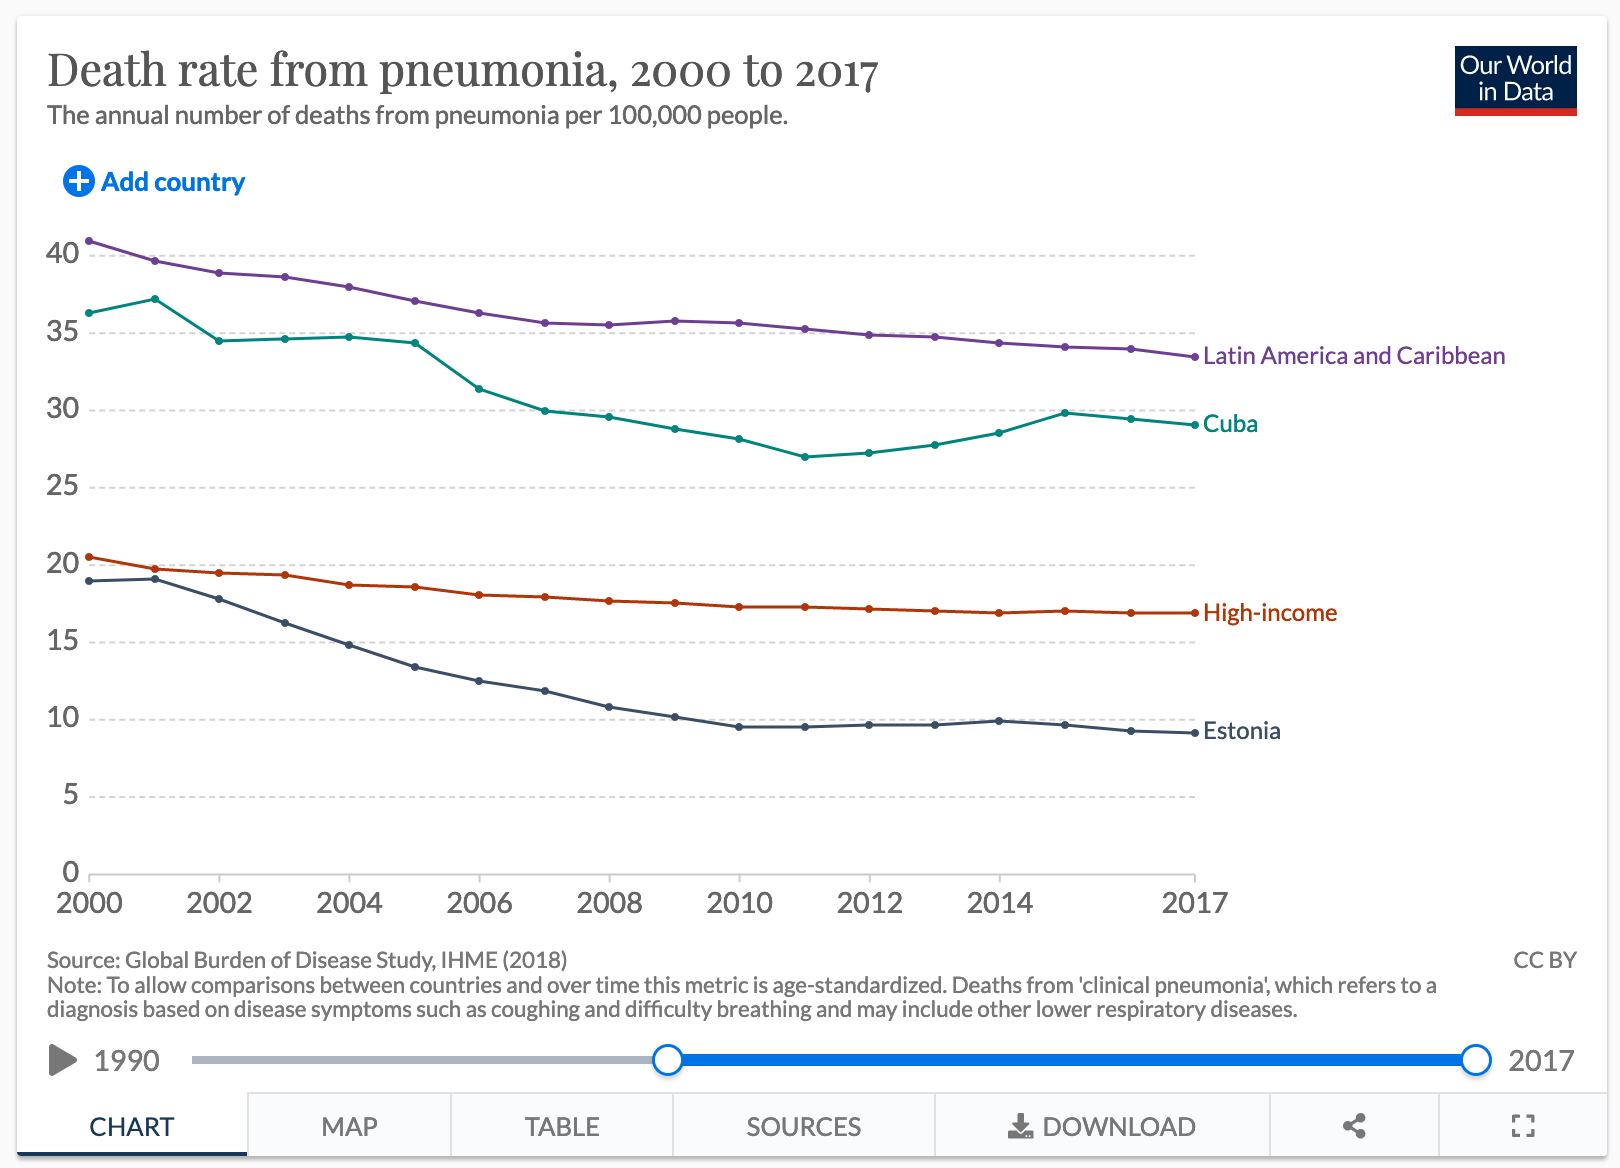
\includegraphics[width=0.99\linewidth]{imagenes/mortalidad-neumonia} \end{center}

Considera los siguientes puntos:

\begin{itemize}
\tightlist
\item
  Las tasas anteriores han sido calculadas con un método que incorpora
  la estructura demográfica de cada país y la estandariza con respecto a
  la pirámide poblacional mundial. En nuestro ejemplo, nuestras tasas no
  serán ajustada de tal forma (este método se conoce en inglés como
  \emph{age-standarized mortality rates}).
\item
  Las tasas reportadas tienen una base distinta, pues son reportadas con
  respecto a una población de 100,000 habitantes. Es decir, son tasas de
  mortalidad anuales para poblaciones de 100K habitantes. Por ejemplo,
  un valor de 5 significa que en promedio 5 habitantes por cada 100K
  mueren de neumonia al año.
\end{itemize}

\textbf{Pregunta 9)} Con esto en mente, escribe los límites necesarios
para encontrar una distribución Gamma adecuada. Encuentra la solución al
sistema de ecuaciones no lineales por medio de la función
\texttt{nleqslv::nleqslv}. Escribe tu razonamiento para seleccionar
dichos valores.

La tasa de habitantes fallecidos por neumonía (filtrado por años tomando
en cuenta únicamente del año \(2015\) hasta el \(2017\)) presenta un
comportamiento uniforme (no en el sentido estricto, pero sí de una forma
bastante aproximada) a lo largo del periodo de estudio en este proyecto
para los distintos grupos de edades, por lo que, se decidió dar como
cota superior el promedio de la tasa de mortalidad para el rango de edad
``\(70+\) years old'', ya que son los máximos alcanzado y como límite
inferior el promedio de las tasa del rango ``\(5-14\) years old'', pues
son las mínimas observadas.

\begin{Shaded}
\begin{Highlighting}[]
\NormalTok{cot_sup <-}\StringTok{ }\KeywordTok{mean}\NormalTok{(}\KeywordTok{c}\NormalTok{(}\FloatTok{184.31}\NormalTok{, }\FloatTok{181.42}\NormalTok{, }\FloatTok{178.51}\NormalTok{))}
\NormalTok{cot_min <-}\StringTok{ }\KeywordTok{mean}\NormalTok{(}\KeywordTok{c}\NormalTok{(}\FloatTok{1.14}\NormalTok{, }\FloatTok{1.12}\NormalTok{, }\FloatTok{1.12}\NormalTok{))}

\NormalTok{limits <-}\StringTok{ }\KeywordTok{c}\NormalTok{(cot_min, cot_sup)}\OperatorTok{/}\NormalTok{(}\DecValTok{10}\OperatorTok{**}\DecValTok{5}\NormalTok{)}

\NormalTok{gamma.limits <-}\StringTok{ }\ControlFlowTok{function}\NormalTok{(x)\{}
  \CommentTok{# reparametrizamos para que el problema sea mas "fácil" en términos numéricos.}
\NormalTok{  log_alpha <-}\StringTok{ }\NormalTok{x[}\DecValTok{1}\NormalTok{]}
\NormalTok{  log_beta  <-}\StringTok{ }\NormalTok{x[}\DecValTok{2}\NormalTok{]}
  
  \CommentTok{# definimos las cotas de probabilidad}
\NormalTok{  p_cota <-}\StringTok{ }\FloatTok{0.1}
  \KeywordTok{c}\NormalTok{(    }\KeywordTok{pgamma}\NormalTok{(limits[}\DecValTok{1}\NormalTok{], }\KeywordTok{exp}\NormalTok{(log_alpha), }\DataTypeTok{rate =} \KeywordTok{exp}\NormalTok{(log_beta)) }\OperatorTok{-}\StringTok{ }\NormalTok{p_cota,}
    \DecValTok{1} \OperatorTok{-}\StringTok{ }\KeywordTok{pgamma}\NormalTok{(limits[}\DecValTok{2}\NormalTok{], }\KeywordTok{exp}\NormalTok{(log_alpha), }\DataTypeTok{rate =} \KeywordTok{exp}\NormalTok{(log_beta)) }\OperatorTok{-}\StringTok{ }\NormalTok{p_cota)}
\NormalTok{\}}

\NormalTok{initial_guess <-}\StringTok{ }\KeywordTok{c}\NormalTok{(}\KeywordTok{log}\NormalTok{(}\DecValTok{1}\NormalTok{), }\KeywordTok{log}\NormalTok{(}\DecValTok{1}\NormalTok{))}

\NormalTok{results <-}\StringTok{ }\KeywordTok{nleqslv}\NormalTok{(initial_guess, gamma.limits)}

\NormalTok{params.prior <-}\StringTok{ }\KeywordTok{exp}\NormalTok{(results}\OperatorTok{$}\NormalTok{x)}

\KeywordTok{rm}\NormalTok{(cot_sup, cot_min, results)}
\end{Highlighting}
\end{Shaded}

\textbf{Pregunta 10)} Grafica los histogramas de una variable aleatoria
Gamma con los valores iniciales para el problema de optimización y con
los finales de dicho algorimo. Esto te servirá de verificación que el
método funciona adecuadamente.

\begin{Shaded}
\begin{Highlighting}[]
\KeywordTok{set.seed}\NormalTok{(}\KeywordTok{min}\NormalTok{(claves_unicas))}

\NormalTok{n_sim <-}\StringTok{ }\DecValTok{5000}
\NormalTok{g_priori_}\DecValTok{1}\NormalTok{ <-}\StringTok{ }\KeywordTok{rgamma}\NormalTok{(n_sim, initial_guess[}\DecValTok{1}\NormalTok{], initial_guess[}\DecValTok{2}\NormalTok{])}
\NormalTok{g_priori_}\DecValTok{2}\NormalTok{ <-}\StringTok{ }\KeywordTok{rgamma}\NormalTok{(n_sim, params.prior[}\DecValTok{1}\NormalTok{], params.prior[}\DecValTok{2}\NormalTok{])}

\NormalTok{data_gamma <-}\StringTok{ }
\StringTok{  }\KeywordTok{data.frame}\NormalTok{(}\DataTypeTok{update =} \KeywordTok{c}\NormalTok{( }\KeywordTok{rep}\NormalTok{(}\StringTok{"Tipo 1"}\NormalTok{, n_sim), }
                       \KeywordTok{rep}\NormalTok{(}\StringTok{"Tipo 2"}\NormalTok{,n_sim)),}
  \DataTypeTok{value =} \KeywordTok{c}\NormalTok{(g_priori_}\DecValTok{1}\NormalTok{, g_priori_}\DecValTok{2}\NormalTok{))}

\NormalTok{data_gamma }\OperatorTok
\StringTok{  }\KeywordTok{ggplot}\NormalTok{(}\KeywordTok{aes}\NormalTok{(}\DataTypeTok{x =}\NormalTok{ value, }\DataTypeTok{fill =}\NormalTok{ update)) }\OperatorTok{+}
\StringTok{  }\KeywordTok{geom_histogram}\NormalTok{(}\DataTypeTok{alpha=}\FloatTok{0.3}\NormalTok{, }\DataTypeTok{position =} \StringTok{'identity'}\NormalTok{, }\DataTypeTok{bins =} \DecValTok{30}\NormalTok{) }\OperatorTok{+}
\StringTok{  }\CommentTok{# scale_fill_manual(values=c("#69b3a2", "#404080")) +}
\StringTok{  }\KeywordTok{xlab}\NormalTok{(}\StringTok{"Tasas de mortalidad por neuomonia"}\NormalTok{) }\OperatorTok{+}
\StringTok{  }\KeywordTok{ylab}\NormalTok{(}\StringTok{"Frecuencia absoluta"}\NormalTok{) }\OperatorTok{+}
\StringTok{  }\KeywordTok{ggtitle}\NormalTok{(}\StringTok{'Simulaciones para distribucion A-priori'}\NormalTok{)}
\end{Highlighting}
\end{Shaded}

\begin{center}\includegraphics[width=0.99\linewidth]{examen-final-alumos-entrega_files/figure-latex/histogramas elicitacion-1} \end{center}

En comparación de las distribuciones apriori, observamos que la segunda
(``Tipo 2''), tiene un mejor comportamiento en comparación con la
primera, que indica que no habrá ninguna muerte con neumonía, en
contraste los datos no lo indican así.

\textbf{Pregunta 11)} ¿Cómo se compara la distribución a priori con las
tasas observadas en los municipios? Puedes utilizar histogramas para
estas comparaciones. Por otro lado, no te preocupes si no se ven
identicas. El punto es ver que nuestras creencias iniciales se ven
coherentes.

\begin{Shaded}
\begin{Highlighting}[]
\NormalTok{data_neum <-}\StringTok{ }\NormalTok{full_data }\OperatorTok\StringTok{ }
\StringTok{  }\KeywordTok{filter}\NormalTok{(municipio }\OperatorTok{!=}\StringTok{ }\DecValTok{999}\NormalTok{) }\OperatorTok\StringTok{ }
\StringTok{  }\KeywordTok{ungroup}\NormalTok{() }\OperatorTok
\StringTok{  }\KeywordTok{select}\NormalTok{(tasa_mort)}

\KeywordTok{data.frame}\NormalTok{(}\DataTypeTok{muertes =} \KeywordTok{c}\NormalTok{(data_neum}\OperatorTok{$}\NormalTok{tasa_mort, }
\NormalTok{                       g_priori_}\DecValTok{2}\NormalTok{),}
           \DataTypeTok{tipo =} \KeywordTok{c}\NormalTok{(}\KeywordTok{rep}\NormalTok{(}\StringTok{'Historico'}\NormalTok{, }\KeywordTok{length}\NormalTok{(data_neum}\OperatorTok{$}\NormalTok{tasa_mort)), }
                    \KeywordTok{rep}\NormalTok{(}\StringTok{'Simulado'}\NormalTok{, n_sim))) }\OperatorTok\StringTok{ }
\StringTok{  }\KeywordTok{ggplot}\NormalTok{(}\KeywordTok{aes}\NormalTok{(}\DataTypeTok{x =}\NormalTok{ muertes, }\DataTypeTok{fill =}\NormalTok{ tipo)) }\OperatorTok{+}\StringTok{ }
\StringTok{  }\KeywordTok{geom_histogram}\NormalTok{(}\DataTypeTok{alpha=}\FloatTok{0.5}\NormalTok{, }\DataTypeTok{position =} \StringTok{'identity'}\NormalTok{) }\OperatorTok{+}
\StringTok{  }\KeywordTok{xlab}\NormalTok{(}\StringTok{'Defunciones por neumonia'}\NormalTok{) }\OperatorTok{+}
\StringTok{  }\KeywordTok{ylab}\NormalTok{(}\StringTok{'Frecuencia absoluta'}\NormalTok{) }\OperatorTok{+}
\StringTok{  }\KeywordTok{ggtitle}\NormalTok{(}\StringTok{'Simulacion VS Historico'}\NormalTok{)}
\end{Highlighting}
\end{Shaded}

\begin{center}\includegraphics[width=0.99\linewidth]{examen-final-alumos-entrega_files/figure-latex/unnamed-chunk-4-1} \end{center}

\begin{Shaded}
\begin{Highlighting}[]
\KeywordTok{rm}\NormalTok{(data_gamma, data_neum, g_priori_}\DecValTok{1}\NormalTok{, g_priori_}\DecValTok{2}\NormalTok{)}
\end{Highlighting}
\end{Shaded}

Se sobreestima la tasa de mortalidad por neumonía para el valor \(0\),
es decir, nuestra distribución apriori supone una gran supervivencia, lo
cual no es respaldado por los datos, sin embargo, eso buscaremos cambiar
incorporando la información de los datos con la distribución posterior.

\textbf{Pregunta 12)} Utiliza un gráfico de dispersión para comparar las
tasas observadas contra la población del municipio. ¿Qué observas?
Utiliza los ejes en escala logaritmica. Para esto checa la función:
\texttt{ggplot2::scale\_x\_log10} y \texttt{ggplot2::scale\_y\_log10}

\begin{Shaded}
\begin{Highlighting}[]
\NormalTok{full_data }\OperatorTok
\StringTok{  }\KeywordTok{ggplot}\NormalTok{(}\KeywordTok{aes}\NormalTok{(}\DataTypeTok{x =}\NormalTok{ tasa_mort, }\DataTypeTok{y =}\NormalTok{ pob_tot)) }\OperatorTok{+}
\StringTok{  }\KeywordTok{geom_point}\NormalTok{(}\DataTypeTok{color =} \StringTok{'tomato'}\NormalTok{) }\OperatorTok{+}
\StringTok{  }\KeywordTok{xlab}\NormalTok{(}\StringTok{'Tasa de mortalidad'}\NormalTok{) }\OperatorTok{+}
\StringTok{  }\KeywordTok{ylab}\NormalTok{(}\StringTok{'Poblacion total'}\NormalTok{) }\OperatorTok{+}
\StringTok{  }\KeywordTok{ggtitle}\NormalTok{(}\StringTok{'Informacion a nivel municipio'}\NormalTok{)}
\end{Highlighting}
\end{Shaded}

\begin{center}\includegraphics[width=0.99\linewidth]{examen-final-alumos-entrega_files/figure-latex/unnamed-chunk-5-1} \end{center}

\begin{Shaded}
\begin{Highlighting}[]
\NormalTok{full_data }\OperatorTok
\StringTok{  }\KeywordTok{ggplot}\NormalTok{(}\KeywordTok{aes}\NormalTok{(}\DataTypeTok{x =}\NormalTok{ tasa_mort, }\DataTypeTok{y =}\NormalTok{ pob_tot)) }\OperatorTok{+}
\StringTok{  }\KeywordTok{geom_point}\NormalTok{(}\DataTypeTok{color =} \StringTok{'tomato'}\NormalTok{) }\OperatorTok{+}
\StringTok{  }\NormalTok{ggplot2}\OperatorTok{::}\KeywordTok{scale_x_log10}\NormalTok{() }\OperatorTok{+}
\StringTok{  }\NormalTok{ggplot2}\OperatorTok{::}\KeywordTok{scale_y_log10}\NormalTok{() }\OperatorTok{+}
\StringTok{  }\KeywordTok{xlab}\NormalTok{(}\StringTok{'Tasa de mortalidad (log)'}\NormalTok{) }\OperatorTok{+}
\StringTok{  }\KeywordTok{ylab}\NormalTok{(}\StringTok{'Poblacion total (log)'}\NormalTok{) }\OperatorTok{+}
\StringTok{  }\KeywordTok{ggtitle}\NormalTok{(}\StringTok{'Informacion a nivel municipio'}\NormalTok{)}
\end{Highlighting}
\end{Shaded}

\begin{center}\includegraphics[width=0.99\linewidth]{examen-final-alumos-entrega_files/figure-latex/unnamed-chunk-5-2} \end{center}

El primer gráfico es un poco ``difícil'' (las palabras difícil, fácil,
sencillo,\ldots{} son demasiado relativa a las características
intrínsecas de los individuos) de asimilar, pues hay una gran
concentración de puntos que no permiten analizar un poco el fenómeno a
similar. Sin embargo, para el segundo gráfico la historia es un
distinta, ya que, pareciese que este fenómeno sigue un comportamiento un
tatnto exponencial, para tasas de mortalidad bajas, la población total
es alta, mientras qeu para tasas de mortalidad altas, la población es
baja. Todo esto con un comportamiento exponencial. Que se presente este
caso, nos da la siguiente idea intuitiva: * La neumonía no afecta de
manera uniforme a la población, pues dependiendo de la estructura
demográfica (en cuanto a edades) de la población, la nuemonía afectará
de manera distinta a cada uno de los distintos grupos.

Cuando tenemos tamaños de población grande, la presencia de muertes por
neumonía es alta, debido a la alta densidad poblacional y de manera
inversa, cuando tenemos tamaños de población bajos, la presencia de
muertes por neumonía es alta, debido a la baja densidad poblacional. Es
relvante mencionar que tenemos presencia de valores atípicos en las
colas, los cuales hacen que nuestra ``hipótesis'' sea falsa.

\textbf{Pregunta 13)} Ahora usaremos la distribución predictiva
\textbf{previa} para explorar los posibles valores que tendrían los
casos de muerte bajo nuestro modelo para municipios de distintos
tamaños. Para este punto considera que la predictiva es una mezcla de
Poisson con Gamma, como se expresa en

\[p(y|n) = \int \textsf{Poisson}(y | n, \theta) \, \textsf{Gamma}(\theta|\alpha, \beta) \, \text{d}\theta.\]
o bien, la forma en especifico de la predictiva preevia. ¡Esto ya lo has
resuelto en la primera parte del examen!

Usa histogramas para ver los números de muertes en municipios
hipotéticos de tamaño \(n = 10^3, 10^4, 10^5.\)

\begin{center}\includegraphics[width=0.99\linewidth]{examen-final-alumos-entrega_files/figure-latex/unnamed-chunk-6-1} \end{center}

\begin{center}\includegraphics[width=0.99\linewidth]{examen-final-alumos-entrega_files/figure-latex/unnamed-chunk-6-2} \end{center}

\begin{center}\includegraphics[width=0.99\linewidth]{examen-final-alumos-entrega_files/figure-latex/unnamed-chunk-6-3} \end{center}

\begin{center}\includegraphics[width=0.99\linewidth]{examen-final-alumos-entrega_files/figure-latex/unnamed-chunk-6-4} \end{center}

\begin{verbatim}
## $y
## [1] "Frecuencia absoluta"
## 
## attr(,"class")
## [1] "labels"
\end{verbatim}

\textbf{Pregunta 14)} Calcula los valores posteriores de las tasas de
mortalidad bajo nuestro modelo bayesiano y compara con los estimadores
de máxima verosimilitud. Para esto puedes utilizar un gráfico de
dispersión cómo el visto en clase o los anteriores. ¿Observas
regularización en nuestras estimaciones? ¿Qué observas si haces un
grafico como el de la pregunta 12?

\[p(y|n) = \int \textsf{Poisson}(y | n, \theta) \, \textsf{Gamma}(\theta|\alpha, \beta) \, \text{d}\theta.\]

Cabe mencionar que la distribución predictiva posterior es la siguiente:

\[ y | n \sim BN(\alpha \text{ } + \text{ } \sum_{i=1}^nx_i, \text{ } \beta \text{ } + \text{ }n)  \]

\begin{Shaded}
\begin{Highlighting}[]
\KeywordTok{set.seed}\NormalTok{(}\KeywordTok{min}\NormalTok{(claves_unicas))}

\NormalTok{full_data_filt <-}\StringTok{ }\NormalTok{full_data }\OperatorTok\StringTok{ }
\StringTok{  }\KeywordTok{filter}\NormalTok{(municipio }\OperatorTok{!=}\StringTok{ }\DecValTok{999}\NormalTok{)}

\NormalTok{calcular_pars_posterior <-}\StringTok{ }\ControlFlowTok{function}\NormalTok{(num_muertes , tam_pob, params.prior)\{}
  
  \CommentTok{# Parametros iniciales}
\NormalTok{  alpha_prior <-}\StringTok{ }\NormalTok{params.prior[}\DecValTok{1}\NormalTok{]}
\NormalTok{  beta_prior <-}\StringTok{ }\NormalTok{params.prior[}\DecValTok{2}\NormalTok{]}
  
  \CommentTok{# Parámetros}
\NormalTok{  alpha_post <-}\StringTok{ }\NormalTok{alpha_prior }\OperatorTok{+}\StringTok{ }\NormalTok{num_muertes}
  
  \CommentTok{# beta post}
\NormalTok{  beta_post <-}\StringTok{ }\NormalTok{beta_prior }\OperatorTok{+}\StringTok{ }\NormalTok{tam_pob}
  \CommentTok{# beta_post <- beta_prior + 1}
  \KeywordTok{return}\NormalTok{(}\KeywordTok{c}\NormalTok{(alpha_post, beta_post)) }
\NormalTok{  \}}

\NormalTok{pars_post <-}\StringTok{ }\KeywordTok{apply}\NormalTok{(full_data_filt[,}\KeywordTok{c}\NormalTok{(}\StringTok{'muertes_neum'}\NormalTok{, }\StringTok{'pob_tot'}\NormalTok{)], }\DecValTok{1}\NormalTok{, }
             \ControlFlowTok{function}\NormalTok{(x) }\KeywordTok{calcular_pars_posterior}\NormalTok{(x[}\DecValTok{1}\NormalTok{], x[}\DecValTok{2}\NormalTok{],}
\NormalTok{                                                 params.prior)) }\OperatorTok\StringTok{ }
\StringTok{  }\KeywordTok{t}\NormalTok{()}

\NormalTok{full_data_filt}\OperatorTok{$}\NormalTok{tasa_sim_post <-}\StringTok{  }\KeywordTok{apply}\NormalTok{(pars_post, }\DecValTok{1}\NormalTok{, }
                                       \ControlFlowTok{function}\NormalTok{(x) }\KeywordTok{rgamma}\NormalTok{(}\DecValTok{1}\NormalTok{, x[}\DecValTok{1}\NormalTok{], x[}\DecValTok{2}\NormalTok{]))}

\NormalTok{full_data_filt }\OperatorTok\StringTok{ }
\StringTok{  }\KeywordTok{ggplot}\NormalTok{(}\KeywordTok{aes}\NormalTok{(}\DataTypeTok{x =}\NormalTok{ tasa_sim_post, }\DataTypeTok{y =}\NormalTok{ tasa_mort)) }\OperatorTok{+}
\StringTok{  }\KeywordTok{geom_point}\NormalTok{() }\OperatorTok{+}
\StringTok{  }\KeywordTok{xlab}\NormalTok{(}\StringTok{'Tasa de mortalidad simulada'}\NormalTok{) }\OperatorTok{+}
\StringTok{  }\KeywordTok{ylab}\NormalTok{(}\StringTok{'Tasa de mortalidad observada'}\NormalTok{) }\OperatorTok{+}
\StringTok{  }\KeywordTok{ggtitle}\NormalTok{(}\StringTok{'Ajuste de simulacion'}\NormalTok{)}
\end{Highlighting}
\end{Shaded}

\begin{center}\includegraphics[width=0.99\linewidth]{examen-final-alumos-entrega_files/figure-latex/unnamed-chunk-7-1} \end{center}

\begin{Shaded}
\begin{Highlighting}[]
\NormalTok{full_data_filt }\OperatorTok\StringTok{ }
\StringTok{  }\KeywordTok{ggplot}\NormalTok{(}\KeywordTok{aes}\NormalTok{(}\DataTypeTok{x =}\NormalTok{ tasa_sim_post, }\DataTypeTok{y =}\NormalTok{ tasa_mort)) }\OperatorTok{+}
\StringTok{  }\KeywordTok{geom_point}\NormalTok{() }\OperatorTok{+}
\StringTok{  }\NormalTok{ggplot2}\OperatorTok{::}\KeywordTok{scale_x_log10}\NormalTok{() }\OperatorTok{+}
\StringTok{  }\NormalTok{ggplot2}\OperatorTok{::}\KeywordTok{scale_y_log10}\NormalTok{() }\OperatorTok{+}
\StringTok{  }\KeywordTok{xlab}\NormalTok{(}\StringTok{'Tasa de mortalidad simulada (log)'}\NormalTok{) }\OperatorTok{+}
\StringTok{  }\KeywordTok{ylab}\NormalTok{(}\StringTok{'Tasa de mortalidad observada (log)'}\NormalTok{) }\OperatorTok{+}
\StringTok{  }\KeywordTok{ggtitle}\NormalTok{(}\StringTok{'Ajuste de simulacion - escala logaritmica'}\NormalTok{)}
\end{Highlighting}
\end{Shaded}

\begin{center}\includegraphics[width=0.99\linewidth]{examen-final-alumos-entrega_files/figure-latex/unnamed-chunk-7-2} \end{center}

\begin{Shaded}
\begin{Highlighting}[]
\CommentTok{# data.frame(tasa_mort = c(full_data_filt$tasa_mort, }
\CommentTok{#                          full_data_filt$tasa_sim_post)) %>% }
\CommentTok{#   mutate(Tipo = c(rep('Observada', 2462), }
\CommentTok{#                   rep('Sim posterior', 2462))) %>% }
\CommentTok{#   ggplot(aes(x = tasa_mort, fill = Tipo)) +}
\CommentTok{#   geom_histogram(alpha = 0.5) +}
\CommentTok{#   xlab('Tasa de mortalidad') +}
\CommentTok{#   ylab('Frecuencia absoluta') +}
\CommentTok{#   ggtitle('Comparacion de simulacion')}


\NormalTok{full_data_filt}\OperatorTok{$}\NormalTok{tasa_sim_ver <-}\StringTok{ }\NormalTok{full_data_filt}\OperatorTok{$}\NormalTok{muertes_neum}\OperatorTok{/}\NormalTok{full_data_filt}\OperatorTok{$}\NormalTok{pob_tot}

\KeywordTok{data.frame}\NormalTok{(}\DataTypeTok{tasa_mort =} \KeywordTok{c}\NormalTok{(full_data_filt}\OperatorTok{$}\NormalTok{tasa_sim_ver, }
\NormalTok{                         full_data_filt}\OperatorTok{$}\NormalTok{tasa_sim_post)) }\OperatorTok\StringTok{ }
\StringTok{  }\KeywordTok{mutate}\NormalTok{(}\DataTypeTok{Tipo =} \KeywordTok{c}\NormalTok{(}\KeywordTok{rep}\NormalTok{(}\StringTok{'Sim Max Ver'}\NormalTok{, }\DecValTok{2456}\NormalTok{), }
                  \KeywordTok{rep}\NormalTok{(}\StringTok{'Sim posterior'}\NormalTok{, }\DecValTok{2456}\NormalTok{))) }\OperatorTok\StringTok{ }
\StringTok{  }\KeywordTok{ggplot}\NormalTok{(}\KeywordTok{aes}\NormalTok{(}\DataTypeTok{x =}\NormalTok{ tasa_mort, }\DataTypeTok{fill =}\NormalTok{ Tipo)) }\OperatorTok{+}
\StringTok{  }\KeywordTok{geom_histogram}\NormalTok{(}\DataTypeTok{alpha =} \FloatTok{0.5}\NormalTok{) }\OperatorTok{+}
\StringTok{  }\KeywordTok{xlab}\NormalTok{(}\StringTok{'Tasa de mortalidad'}\NormalTok{) }\OperatorTok{+}
\StringTok{  }\KeywordTok{ylab}\NormalTok{(}\StringTok{'Frecuencia absoluta'}\NormalTok{) }\OperatorTok{+}
\StringTok{  }\KeywordTok{ggtitle}\NormalTok{(}\StringTok{'Comparacion de simulacion'}\NormalTok{)}
\end{Highlighting}
\end{Shaded}

\begin{center}\includegraphics[width=0.99\linewidth]{examen-final-alumos-entrega_files/figure-latex/unnamed-chunk-7-3} \end{center}

Notemos un hecho importante en la gráfica ``Ajuste por simulación escala
logarítmica'', el cual es que para las tasas de mortalidad simuladas más
altas, se vienen las tasas de mortalidad observadas más altas y de
manera análoga para las más chicas. Esto es importante, pues si no fuese
así, estaríamos llegando a contradicciones en el estudio. En comparación
con los estimadores de máxima verosimilitud con los parámetros obtenidos
por la distribución posterior, observamos que las distribuciones tienen
la misma ``forma'', mas con el gran cambio en que para la máxima
verosimilitud hay una mayor frecuencia pra las tasas más bajas a
comparación de la posterior.

\textbf{Pregunta 15)} Utiliza la distribución predictiva
\emph{posterior} para verificar el ajuste del modelo. Para esto, escoge
tres municipios al azar de distintos tamaños (chico, mediano, grande)
Grafica un histograma y compara con el número observado de defunciones.

\begin{Shaded}
\begin{Highlighting}[]
\KeywordTok{set.seed}\NormalTok{(}\KeywordTok{min}\NormalTok{(claves_unicas))}

\NormalTok{full_data_filt <-}\StringTok{ }\NormalTok{full_data_filt }\OperatorTok\StringTok{ }
\StringTok{  }\KeywordTok{mutate}\NormalTok{(}\DataTypeTok{tamanio =} \KeywordTok{ifelse}\NormalTok{(pob_tot }\OperatorTok{<=}\StringTok{ }\DecValTok{1000}\NormalTok{, }\DecValTok{1}\NormalTok{, }
                          \KeywordTok{ifelse}\NormalTok{(pob_tot }\OperatorTok{<=}\StringTok{ }\DecValTok{10000}\NormalTok{, }\DecValTok{2}\NormalTok{, }\DecValTok{3}\NormalTok{)))}

\NormalTok{full_data_filt }\OperatorTok\StringTok{ }
\StringTok{  }\KeywordTok{group_by}\NormalTok{(tamanio) }\OperatorTok\StringTok{ }
\StringTok{  }\KeywordTok{summarise}\NormalTok{(}\DataTypeTok{count =} \KeywordTok{n}\NormalTok{())}
\end{Highlighting}
\end{Shaded}

\begin{verbatim}
## # A tibble: 3 x 2
##   tamanio count
##     <dbl> <int>
## 1       1   128
## 2       2   951
## 3       3  1377
\end{verbatim}

\begin{Shaded}
\begin{Highlighting}[]
\NormalTok{pos_chico <-}\StringTok{ }\KeywordTok{sample}\NormalTok{(}\KeywordTok{which}\NormalTok{(full_data_filt}\OperatorTok{$}\NormalTok{tamanio }\OperatorTok{==}\StringTok{ }\DecValTok{1}\NormalTok{), }\DecValTok{1}\NormalTok{)}
\NormalTok{pos_mediano <-}\StringTok{ }\KeywordTok{sample}\NormalTok{(}\KeywordTok{which}\NormalTok{(full_data_filt}\OperatorTok{$}\NormalTok{tamanio }\OperatorTok{==}\StringTok{ }\DecValTok{2}\NormalTok{), }\DecValTok{1}\NormalTok{)}
\NormalTok{pos_grande <-}\StringTok{ }\KeywordTok{sample}\NormalTok{(}\KeywordTok{which}\NormalTok{(full_data_filt}\OperatorTok{$}\NormalTok{tamanio }\OperatorTok{==}\StringTok{ }\DecValTok{3}\NormalTok{), }\DecValTok{1}\NormalTok{)}

\NormalTok{par_post_chico <-}\StringTok{ }\NormalTok{pars_post[pos_chico,]}
\NormalTok{par_post_mediano <-}\StringTok{ }\NormalTok{pars_post[pos_mediano,]}
\NormalTok{par_post_grande <-}\StringTok{ }\NormalTok{pars_post[pos_grande,]}


\KeywordTok{data.frame}\NormalTok{(}\DataTypeTok{sim =} \KeywordTok{rnbinom}\NormalTok{(}\DecValTok{1000}\NormalTok{, }
                    \DataTypeTok{size =}\NormalTok{ par_post_chico[}\DecValTok{2}\NormalTok{]}\OperatorTok{*}\NormalTok{(params.prior[}\DecValTok{1}\NormalTok{]) }\OperatorTok{+}\StringTok{ }\NormalTok{par_post_chico[}\DecValTok{1}\NormalTok{],}
                    \DataTypeTok{prob =}\NormalTok{ (params.prior[}\DecValTok{2}\NormalTok{] }\OperatorTok{+}\StringTok{ }\DecValTok{1}\NormalTok{)}\OperatorTok{/}\NormalTok{(params.prior[}\DecValTok{2}\NormalTok{] }\OperatorTok{+}\StringTok{ }\DecValTok{1} \OperatorTok{+}\StringTok{ }\DecValTok{1}\NormalTok{) )) }\OperatorTok\StringTok{ }
\StringTok{  }\KeywordTok{ggplot}\NormalTok{(}\KeywordTok{aes}\NormalTok{(}\DataTypeTok{x =}\NormalTok{ sim)) }\OperatorTok{+}
\StringTok{  }\KeywordTok{geom_histogram}\NormalTok{() }\OperatorTok{+}
\StringTok{  }\KeywordTok{geom_vline}\NormalTok{(}\DataTypeTok{xintercept =}\NormalTok{ par_post_chico[}\DecValTok{1}\NormalTok{], }\DataTypeTok{color =} \StringTok{'red'}\NormalTok{) }\OperatorTok{+}
\StringTok{  }\KeywordTok{geom_text}\NormalTok{(}\KeywordTok{aes}\NormalTok{(}\DataTypeTok{x=}\FloatTok{2.8}\NormalTok{, }\DataTypeTok{y=}\DecValTok{350}\NormalTok{,}
                \DataTypeTok{label=}\StringTok{"Defunciones observadas"}\NormalTok{), }
            \DataTypeTok{colour=}\StringTok{"black"}\NormalTok{, }\DataTypeTok{vjust =} \FloatTok{1.2}\NormalTok{) }\OperatorTok{+}
\StringTok{  }\KeywordTok{xlab}\NormalTok{(}\StringTok{'Defunciones por neumonia'}\NormalTok{) }\OperatorTok{+}
\StringTok{  }\KeywordTok{ylab}\NormalTok{(}\StringTok{'Frecuencia absoluta'}\NormalTok{) }\OperatorTok{+}
\StringTok{  }\KeywordTok{ggtitle}\NormalTok{(}\StringTok{'Simulacion defunciones por neumonia'}\NormalTok{) }\OperatorTok{+}
\StringTok{  }\KeywordTok{labs}\NormalTok{(}\DataTypeTok{subtitle =} \StringTok{'Municipio de tamanio pequenio'}\NormalTok{)}
\end{Highlighting}
\end{Shaded}

\begin{center}\includegraphics[width=0.99\linewidth]{examen-final-alumos-entrega_files/figure-latex/unnamed-chunk-8-1} \end{center}

\begin{Shaded}
\begin{Highlighting}[]
\KeywordTok{data.frame}\NormalTok{(}\DataTypeTok{sim =} \KeywordTok{rnbinom}\NormalTok{(}\DecValTok{1000}\NormalTok{, }
                    \DataTypeTok{size =}\NormalTok{ par_post_mediano[}\DecValTok{2}\NormalTok{]}\OperatorTok{*}\NormalTok{(par_post_mediano[}\DecValTok{1}\NormalTok{]) }\OperatorTok{+}\StringTok{ }\NormalTok{par_post_mediano[}\DecValTok{1}\NormalTok{],}
                    \DataTypeTok{prob =}\NormalTok{ (par_post_mediano[}\DecValTok{2}\NormalTok{] }\OperatorTok{+}\StringTok{ }\DecValTok{1}\NormalTok{)}\OperatorTok{/}\NormalTok{(par_post_mediano[}\DecValTok{2}\NormalTok{] }\OperatorTok{+}\StringTok{ }\DecValTok{1} \OperatorTok{+}\StringTok{ }\DecValTok{1}\NormalTok{) )) }\OperatorTok\StringTok{ }
\StringTok{  }\KeywordTok{ggplot}\NormalTok{(}\KeywordTok{aes}\NormalTok{(}\DataTypeTok{x =}\NormalTok{ sim)) }\OperatorTok{+}
\StringTok{  }\KeywordTok{geom_histogram}\NormalTok{() }\OperatorTok{+}
\StringTok{  }\KeywordTok{geom_vline}\NormalTok{(}\DataTypeTok{xintercept =}\NormalTok{ par_post_mediano[}\DecValTok{1}\NormalTok{], }\DataTypeTok{color =} \StringTok{'red'}\NormalTok{) }\OperatorTok{+}
\StringTok{  }\KeywordTok{geom_text}\NormalTok{(}\KeywordTok{aes}\NormalTok{(}\DataTypeTok{x=}\DecValTok{3}\NormalTok{, }\DataTypeTok{y=}\DecValTok{250}\NormalTok{,}
                \DataTypeTok{label=}\StringTok{"Defunciones observadas"}\NormalTok{), }
            \DataTypeTok{colour=}\StringTok{"black"}\NormalTok{, }\DataTypeTok{vjust =} \FloatTok{1.2}\NormalTok{) }\OperatorTok{+}
\StringTok{  }\KeywordTok{xlab}\NormalTok{(}\StringTok{'Defunciones por neumonia'}\NormalTok{) }\OperatorTok{+}
\StringTok{  }\KeywordTok{ylab}\NormalTok{(}\StringTok{'Frecuencia absoluta'}\NormalTok{) }\OperatorTok{+}
\StringTok{  }\KeywordTok{ggtitle}\NormalTok{(}\StringTok{'Simulacion defunciones por neumonia'}\NormalTok{) }\OperatorTok{+}
\StringTok{  }\KeywordTok{labs}\NormalTok{(}\DataTypeTok{subtitle =} \StringTok{'Municipio de tamanio mediano'}\NormalTok{)}
\end{Highlighting}
\end{Shaded}

\begin{center}\includegraphics[width=0.99\linewidth]{examen-final-alumos-entrega_files/figure-latex/unnamed-chunk-8-2} \end{center}

\begin{Shaded}
\begin{Highlighting}[]
\KeywordTok{data.frame}\NormalTok{(}\DataTypeTok{sim =} \KeywordTok{rnbinom}\NormalTok{(}\DecValTok{1000}\NormalTok{, }
                    \DataTypeTok{size =}\NormalTok{ par_post_grande[}\DecValTok{2}\NormalTok{]}\OperatorTok{*}\NormalTok{(par_post_grande[}\DecValTok{1}\NormalTok{]) }\OperatorTok{+}\StringTok{ }\NormalTok{par_post_grande[}\DecValTok{1}\NormalTok{],}
                    \DataTypeTok{prob =}\NormalTok{ (par_post_grande[}\DecValTok{2}\NormalTok{] }\OperatorTok{+}\StringTok{ }\DecValTok{1}\NormalTok{)}\OperatorTok{/}\NormalTok{(par_post_grande[}\DecValTok{2}\NormalTok{] }\OperatorTok{+}\StringTok{ }\DecValTok{1} \OperatorTok{+}\StringTok{ }\DecValTok{1}\NormalTok{) )) }\OperatorTok\StringTok{ }
\StringTok{  }\KeywordTok{ggplot}\NormalTok{(}\KeywordTok{aes}\NormalTok{(}\DataTypeTok{x =}\NormalTok{ sim)) }\OperatorTok{+}
\StringTok{  }\KeywordTok{geom_histogram}\NormalTok{() }\OperatorTok{+}
\StringTok{  }\KeywordTok{geom_vline}\NormalTok{(}\DataTypeTok{xintercept =}\NormalTok{ par_post_grande[}\DecValTok{1}\NormalTok{], }\DataTypeTok{color =} \StringTok{'red'}\NormalTok{) }\OperatorTok{+}
\StringTok{  }\KeywordTok{geom_text}\NormalTok{(}\KeywordTok{aes}\NormalTok{(}\DataTypeTok{x=}\DecValTok{57}\NormalTok{, }\DataTypeTok{y=}\DecValTok{125}\NormalTok{,}
                \DataTypeTok{label=}\StringTok{"Defunciones observadas"}\NormalTok{), }
            \DataTypeTok{colour=}\StringTok{"black"}\NormalTok{, }\DataTypeTok{vjust =} \FloatTok{1.2}\NormalTok{) }\OperatorTok{+}
\StringTok{  }\KeywordTok{xlab}\NormalTok{(}\StringTok{'Defunciones por neumonia'}\NormalTok{) }\OperatorTok{+}
\StringTok{  }\KeywordTok{ylab}\NormalTok{(}\StringTok{'Frecuencia absoluta'}\NormalTok{) }\OperatorTok{+}
\StringTok{  }\KeywordTok{ggtitle}\NormalTok{(}\StringTok{'Simulacion defunciones por neumonia'}\NormalTok{) }\OperatorTok{+}
\StringTok{  }\KeywordTok{labs}\NormalTok{(}\DataTypeTok{subtitle =} \StringTok{'Municipio de tamanio grande'}\NormalTok{)}
\end{Highlighting}
\end{Shaded}

\begin{center}\includegraphics[width=0.99\linewidth]{examen-final-alumos-entrega_files/figure-latex/unnamed-chunk-8-3} \end{center}

Para las simulaciones de las defunciones por neumonía de cada municipio
notemos que la la cantidad de defunciones observadas se encuentra
alrededor de la media de la distribución.

\hypertarget{incorporando-grupos-de-edad}{%
\subsection{Incorporando Grupos de
Edad}\label{incorporando-grupos-de-edad}}

Se sabe que las muertes por neumonia no son uniformes y las tasas de
mortalidad son mas altas en niños y personas mayores. Ahora realizaremos
el mismo análisis considerando grupos de edad. Para esto ampliaremos
nuestro modelo

\[ y_{k,i} \, | \, n_{k,i}, \theta_{k,i} \sim \textsf{Poisson}(\lambda_{k,i}),\]

donde utilizamos el sub-indice \(k,i\) para denotar el \(k\)-ésimo grupo
de edad en el \(i\)-ésimo municipio.

\textbf{Pregunta 16)} Genera histogramas para cada grupo de edad y
discute si el supuesto anterior esta soportado por los datos. Para esto
calcula las tasas de mortalidad adecuadas. Auxiliate de
\texttt{ggplot2::facet\_wrap}.

\begin{Shaded}
\begin{Highlighting}[]
\NormalTok{datos_edad <-}\StringTok{ }\NormalTok{poblacion }\OperatorTok\StringTok{ }
\StringTok{    }\KeywordTok{select}\NormalTok{(entidad, municipio, p_0a2}\OperatorTok{:}\NormalTok{pob65_mas) }\OperatorTok\StringTok{ }
\StringTok{  }\KeywordTok{pivot_longer}\NormalTok{(p_0a2}\OperatorTok{:}\NormalTok{pob65_mas, }
               \DataTypeTok{names_to =} \StringTok{"GrupoEdad"}\NormalTok{,}
               \DataTypeTok{values_to =} \StringTok{"Poblacion"}\NormalTok{) }\OperatorTok\StringTok{ }
\StringTok{  }\KeywordTok{left_join}\NormalTok{(defunciones }\OperatorTok\StringTok{ }
\StringTok{  }\KeywordTok{group_by}\NormalTok{(entidad, municipio, edad_grupos) }\OperatorTok\StringTok{ }
\StringTok{  }\KeywordTok{count}\NormalTok{(}\DataTypeTok{name=}\StringTok{"Defunciones"}\NormalTok{) }\OperatorTok\StringTok{ }
\StringTok{  }\KeywordTok{mutate}\NormalTok{(}\DataTypeTok{GrupoEdad =} \KeywordTok{recode}\NormalTok{(edad_grupos,}
                            \StringTok{"[0,3)"}\NormalTok{=}\StringTok{"p_0a2"}\NormalTok{,}
                            \StringTok{"[3,6)"}\NormalTok{=}\StringTok{"p_3a5"}\NormalTok{,}
                            \StringTok{"[6,12)"}\NormalTok{=}\StringTok{"p_6a11"}\NormalTok{,}
                            \StringTok{"[12,18)"}\NormalTok{=}\StringTok{"p_12a17"}\NormalTok{,}
                            \StringTok{"[18,25)"}\NormalTok{=}\StringTok{"p_18a24"}\NormalTok{,}
                            \StringTok{"[25,64)"}\NormalTok{=}\StringTok{"p_25a64"}\NormalTok{,}
                            \StringTok{"[64,Inf]"}\NormalTok{=}\StringTok{"pob65_mas"}\NormalTok{)),}
  \DataTypeTok{by=}\KeywordTok{c}\NormalTok{(}\StringTok{'entidad'}\NormalTok{, }\StringTok{'municipio'}\NormalTok{, }\StringTok{'GrupoEdad'}\NormalTok{ )) }\OperatorTok\StringTok{ }
\StringTok{  }\KeywordTok{mutate}\NormalTok{(}\DataTypeTok{Defunciones =} \KeywordTok{replace_na}\NormalTok{(Defunciones, }\DecValTok{0}\NormalTok{),}
    \DataTypeTok{mortalidad =}\NormalTok{ Defunciones}\OperatorTok{/}\NormalTok{Poblacion,}
    \DataTypeTok{GrupoEdad =} \KeywordTok{factor}\NormalTok{(GrupoEdad, }
                       \DataTypeTok{levels =} \KeywordTok{c}\NormalTok{(}\StringTok{"p_0a2"}\NormalTok{,}\StringTok{"p_3a5"}\NormalTok{,}\StringTok{"p_6a11"}\NormalTok{,}\StringTok{"p_12a17"}\NormalTok{,}
                                  \StringTok{"p_18a24"}\NormalTok{,}\StringTok{"p_25a64"}\NormalTok{,}\StringTok{"pob65_mas"}\NormalTok{)))}
\end{Highlighting}
\end{Shaded}

Ahora la grafica

\begin{Shaded}
\begin{Highlighting}[]
\NormalTok{datos_edad }\OperatorTok\StringTok{ }
\StringTok{  }\KeywordTok{ggplot}\NormalTok{() }\OperatorTok{+}
\StringTok{  }\KeywordTok{geom_histogram}\NormalTok{(}\KeywordTok{aes}\NormalTok{(}\DataTypeTok{x=}\NormalTok{mortalidad), }\DataTypeTok{bins=}\DecValTok{40}\NormalTok{) }\OperatorTok{+}
\StringTok{  }\KeywordTok{facet_wrap}\NormalTok{(}\KeywordTok{vars}\NormalTok{(GrupoEdad))}
\end{Highlighting}
\end{Shaded}

\begin{center}\includegraphics[width=0.99\linewidth]{examen-final-alumos-entrega_files/figure-latex/unnamed-chunk-10-1} \end{center}

\begin{Shaded}
\begin{Highlighting}[]
\NormalTok{datos_edad }\OperatorTok\StringTok{ }
\StringTok{  }\KeywordTok{group_by}\NormalTok{(GrupoEdad) }\OperatorTok\StringTok{ }
\StringTok{  }\KeywordTok{summarise}\NormalTok{(}\DataTypeTok{Poblacion =} \KeywordTok{sum}\NormalTok{(Poblacion))}
\end{Highlighting}
\end{Shaded}

\begin{verbatim}
## # A tibble: 7 x 2
##   GrupoEdad Poblacion
##   <fct>         <dbl>
## 1 p_0a2       6157867
## 2 p_3a5       6535234
## 3 p_6a11     13318563
## 4 p_12a17    13215080
## 5 p_18a24    14207435
## 6 p_25a64    50566040
## 7 pob65_mas   6938913
\end{verbatim}

Por motivos de simplicidad usaremos la misma distribución previa para
cada tasa de mortalidad asociada a grupos de edad y municipio que en los
puntos anteriores.

\textbf{Pregunta 17)} Utiliza graficos de dispersión para determinar si
hay efectos de regularización. Las ideas las encuentras arriba en la
pregunta 12 y 14.

\begin{Shaded}
\begin{Highlighting}[]
\NormalTok{vec_gamma <-}\StringTok{ }\KeywordTok{Vectorize}\NormalTok{(rgamma)}
\NormalTok{datos_edad <-}\StringTok{  }\NormalTok{datos_edad }\OperatorTok
\StringTok{  }\KeywordTok{mutate}\NormalTok{(}\DataTypeTok{alpha_post =}\NormalTok{ params.prior[}\DecValTok{1}\NormalTok{] }\OperatorTok{+}\StringTok{ }\NormalTok{Defunciones,}
         \DataTypeTok{beta_post =}\NormalTok{ params.prior[}\DecValTok{2}\NormalTok{] }\OperatorTok{+}\StringTok{ }\NormalTok{Poblacion,}
         \DataTypeTok{theta_post =} \KeywordTok{vec_gamma}\NormalTok{(}\DecValTok{1}\NormalTok{,alpha_post,beta_post))}
\end{Highlighting}
\end{Shaded}

\begin{Shaded}
\begin{Highlighting}[]
\NormalTok{datos_edad }\OperatorTok\StringTok{ }
\StringTok{  }\KeywordTok{ggplot}\NormalTok{() }\OperatorTok{+}
\StringTok{  }\KeywordTok{geom_point}\NormalTok{(}\KeywordTok{aes}\NormalTok{(}\DataTypeTok{x=}\NormalTok{mortalidad, }\DataTypeTok{y =}\NormalTok{ theta_post), }\DataTypeTok{size=}\FloatTok{0.5}\NormalTok{, }\DataTypeTok{alpha=}\FloatTok{0.5}\NormalTok{) }\OperatorTok{+}
\StringTok{  }\KeywordTok{facet_wrap}\NormalTok{(}\KeywordTok{vars}\NormalTok{(GrupoEdad), }\DataTypeTok{scale=}\StringTok{"free"}\NormalTok{)}
\end{Highlighting}
\end{Shaded}

\begin{center}\includegraphics[width=0.99\linewidth]{examen-final-alumos-entrega_files/figure-latex/datos por edad-1} \end{center}

\textbf{Pregunta 18)} Para uno de los tres municipios que escogiste
anteriormente utiliza la distribución predictiva posterior para
verificar el ajuste del modelo para los grupos de edad:
\([0,3), [18,25) \text{ y } [64, \infty).\)

\begin{Shaded}
\begin{Highlighting}[]
\NormalTok{pos_chico <-}\StringTok{ }\KeywordTok{sample}\NormalTok{(}\KeywordTok{which}\NormalTok{(full_data_filt}\OperatorTok{$}\NormalTok{tamanio }\OperatorTok{==}\StringTok{ }\DecValTok{1}\NormalTok{), }\DecValTok{1}\NormalTok{)}
\NormalTok{pos_mediano <-}\StringTok{ }\KeywordTok{sample}\NormalTok{(}\KeywordTok{which}\NormalTok{(full_data_filt}\OperatorTok{$}\NormalTok{tamanio }\OperatorTok{==}\StringTok{ }\DecValTok{2}\NormalTok{), }\DecValTok{1}\NormalTok{)}
\NormalTok{pos_grande <-}\StringTok{ }\KeywordTok{sample}\NormalTok{(}\KeywordTok{which}\NormalTok{(full_data_filt}\OperatorTok{$}\NormalTok{tamanio }\OperatorTok{==}\StringTok{ }\DecValTok{3}\NormalTok{), }\DecValTok{1}\NormalTok{)}

\NormalTok{chico <-}\StringTok{ }\KeywordTok{paste0}\NormalTok{(full_data[pos_chico,}\StringTok{'entidad'}\NormalTok{], }
\NormalTok{                full_data[pos_chico,}\StringTok{'municipio'}\NormalTok{])}
\NormalTok{mediano <-}\StringTok{ }\KeywordTok{paste0}\NormalTok{(full_data[pos_mediano,}\StringTok{'entidad'}\NormalTok{],}
\NormalTok{                  full_data[pos_mediano,}\StringTok{'municipio'}\NormalTok{])}
\NormalTok{grande <-}\StringTok{ }\KeywordTok{paste0}\NormalTok{(full_data[pos_grande,}\StringTok{'entidad'}\NormalTok{], }
\NormalTok{                 full_data[pos_grande,}\StringTok{'municipio'}\NormalTok{])}

\NormalTok{muestra_edad <-}\StringTok{ }\NormalTok{datos_edad }\OperatorTok\StringTok{ }
\StringTok{  }\KeywordTok{mutate}\NormalTok{(}\DataTypeTok{region =} \KeywordTok{paste0}\NormalTok{(entidad, municipio)) }\OperatorTok\StringTok{ }
\StringTok{  }\KeywordTok{filter}\NormalTok{(region }\OperatorTok{==}\StringTok{ }\NormalTok{chico }\OperatorTok{|}\StringTok{ }\NormalTok{region}\OperatorTok{==}\NormalTok{mediano }\OperatorTok{|}\StringTok{ }\NormalTok{region}\OperatorTok{==}\NormalTok{grande) }\OperatorTok\StringTok{ }
\StringTok{  }\KeywordTok{mutate}\NormalTok{(}\DataTypeTok{tamano =} \KeywordTok{factor}\NormalTok{(}\KeywordTok{ifelse}\NormalTok{(region}\OperatorTok{==}\NormalTok{chico,}
                         \StringTok{"chico"}\NormalTok{,}
                         \KeywordTok{ifelse}\NormalTok{(region}\OperatorTok{==}\NormalTok{mediano, }\StringTok{"mediano"}\NormalTok{, }\StringTok{"grande"}\NormalTok{)),}
                         \DataTypeTok{levels =} \KeywordTok{c}\NormalTok{(}\StringTok{"chico"}\NormalTok{, }\StringTok{"mediano"}\NormalTok{, }\StringTok{"grande"}\NormalTok{)))}

\NormalTok{res =}\StringTok{ }\NormalTok{muestra_edad}

\ControlFlowTok{for}\NormalTok{ (i }\ControlFlowTok{in} \DecValTok{1}\OperatorTok{:}\DecValTok{1000}\NormalTok{)\{}
\NormalTok{  res =}\StringTok{ }\KeywordTok{rbind}\NormalTok{(res, muestra_edad)}
\NormalTok{\} }
\NormalTok{  vec_bn <-}\StringTok{ }\KeywordTok{Vectorize}\NormalTok{(rnbinom)}


\NormalTok{res <-}\StringTok{ }\NormalTok{res }\OperatorTok\StringTok{ }
\StringTok{  }\KeywordTok{mutate}\NormalTok{(}\DataTypeTok{sim =} \KeywordTok{vec_bn}\NormalTok{(}\DecValTok{1}\NormalTok{,  }\DataTypeTok{size =}\NormalTok{ Poblacion}\OperatorTok{*}\NormalTok{(params.prior[}\DecValTok{1}\NormalTok{])}\OperatorTok{+}\NormalTok{Defunciones,}
                           \DataTypeTok{prob =}\NormalTok{ (params.prior[}\DecValTok{2}\NormalTok{]}\OperatorTok{+}\DecValTok{1}\NormalTok{)}\OperatorTok{/}\NormalTok{(params.prior[}\DecValTok{2}\NormalTok{]}\OperatorTok{+}\DecValTok{1}\OperatorTok{+}\DecValTok{1}\NormalTok{)))}
\end{Highlighting}
\end{Shaded}

\begin{Shaded}
\begin{Highlighting}[]
\NormalTok{res }\OperatorTok\StringTok{ }
\StringTok{  }\KeywordTok{filter}\NormalTok{(tamano }\OperatorTok{==}\StringTok{ "grande"}\NormalTok{) }\OperatorTok\StringTok{ }
\StringTok{  }\KeywordTok{ggplot}\NormalTok{() }\OperatorTok{+}
\StringTok{  }\KeywordTok{geom_histogram}\NormalTok{(}\KeywordTok{aes}\NormalTok{(}\DataTypeTok{x=}\NormalTok{sim)) }\OperatorTok{+}
\StringTok{  }\KeywordTok{facet_wrap}\NormalTok{(}\OperatorTok{~}\NormalTok{GrupoEdad, }\DataTypeTok{scale =} \StringTok{"free"}\NormalTok{)}
\end{Highlighting}
\end{Shaded}

\begin{center}\includegraphics[width=0.99\linewidth]{examen-final-alumos-entrega_files/figure-latex/Municipio grande-1} \end{center}

\begin{Shaded}
\begin{Highlighting}[]
\NormalTok{muestra_edad }\OperatorTok\StringTok{ }\KeywordTok{filter}\NormalTok{(tamano}\OperatorTok{==}\StringTok{"grande"}\NormalTok{)}
\end{Highlighting}
\end{Shaded}

\begin{verbatim}
## # A tibble: 7 x 12
##   entidad municipio GrupoEdad Poblacion edad_grupos Defunciones mortalidad
##   <chr>   <chr>     <fct>         <dbl> <chr>             <dbl>      <dbl>
## 1 05      033       p_0a2          6150 <NA>                  0  0        
## 2 05      033       p_3a5          6289 <NA>                  0  0        
## 3 05      033       p_6a11        13034 <NA>                  0  0        
## 4 05      033       p_12a17       12782 <NA>                  0  0        
## 5 05      033       p_18a24       11756 <NA>                  0  0        
## 6 05      033       p_25a64       45220 [25,64)               4  0.0000885
## 7 05      033       pob65_mas      7305 [64,Inf]             52  0.00712  
## # ... with 5 more variables: alpha_post <dbl>, beta_post <dbl>,
## #   theta_post <dbl>, region <chr>, tamano <fct>
\end{verbatim}

\begin{Shaded}
\begin{Highlighting}[]
\NormalTok{res }\OperatorTok\StringTok{ }
\StringTok{  }\KeywordTok{filter}\NormalTok{(tamano }\OperatorTok{==}\StringTok{ "mediano"}\NormalTok{) }\OperatorTok\StringTok{ }
\StringTok{  }\KeywordTok{ggplot}\NormalTok{() }\OperatorTok{+}
\StringTok{  }\KeywordTok{geom_histogram}\NormalTok{(}\KeywordTok{aes}\NormalTok{(}\DataTypeTok{x=}\NormalTok{sim)) }\OperatorTok{+}
\StringTok{  }\KeywordTok{facet_wrap}\NormalTok{(}\OperatorTok{~}\NormalTok{GrupoEdad, }\DataTypeTok{scale =} \StringTok{"free"}\NormalTok{)}
\end{Highlighting}
\end{Shaded}

\begin{center}\includegraphics[width=0.99\linewidth]{examen-final-alumos-entrega_files/figure-latex/Municipio mediano-1} \end{center}

\begin{Shaded}
\begin{Highlighting}[]
\NormalTok{muestra_edad }\OperatorTok\StringTok{ }\KeywordTok{filter}\NormalTok{(tamano}\OperatorTok{==}\StringTok{"mediano"}\NormalTok{)}
\end{Highlighting}
\end{Shaded}

\begin{verbatim}
## # A tibble: 7 x 12
##   entidad municipio GrupoEdad Poblacion edad_grupos Defunciones mortalidad
##   <chr>   <chr>     <fct>         <dbl> <chr>             <dbl>      <dbl>
## 1 30      074       p_0a2           378 [0,3)                 1    0.00265
## 2 30      074       p_3a5           363 <NA>                  0    0      
## 3 30      074       p_6a11          806 <NA>                  0    0      
## 4 30      074       p_12a17         762 <NA>                  0    0      
## 5 30      074       p_18a24         802 <NA>                  0    0      
## 6 30      074       p_25a64        3130 <NA>                  0    0      
## 7 30      074       pob65_mas       458 [64,Inf]              4    0.00873
## # ... with 5 more variables: alpha_post <dbl>, beta_post <dbl>,
## #   theta_post <dbl>, region <chr>, tamano <fct>
\end{verbatim}

\begin{Shaded}
\begin{Highlighting}[]
\NormalTok{res }\OperatorTok\StringTok{ }
\StringTok{  }\KeywordTok{filter}\NormalTok{(tamano }\OperatorTok{==}\StringTok{ "chico"}\NormalTok{) }\OperatorTok\StringTok{ }
\StringTok{  }\KeywordTok{ggplot}\NormalTok{() }\OperatorTok{+}
\StringTok{  }\KeywordTok{geom_histogram}\NormalTok{(}\KeywordTok{aes}\NormalTok{(}\DataTypeTok{x=}\NormalTok{sim)) }\OperatorTok{+}
\StringTok{  }\KeywordTok{facet_wrap}\NormalTok{(}\OperatorTok{~}\NormalTok{GrupoEdad, }\DataTypeTok{scale =} \StringTok{"free"}\NormalTok{)}
\end{Highlighting}
\end{Shaded}

\begin{center}\includegraphics[width=0.99\linewidth]{examen-final-alumos-entrega_files/figure-latex/Municipio chico-1} \end{center}

\begin{Shaded}
\begin{Highlighting}[]
\NormalTok{muestra_edad }\OperatorTok\StringTok{ }\KeywordTok{filter}\NormalTok{(tamano}\OperatorTok{==}\StringTok{"chico"}\NormalTok{)}
\end{Highlighting}
\end{Shaded}

\begin{verbatim}
## # A tibble: 7 x 12
##   entidad municipio GrupoEdad Poblacion edad_grupos Defunciones mortalidad
##   <chr>   <chr>     <fct>         <dbl> <chr>             <dbl>      <dbl>
## 1 20      168       p_0a2            55 <NA>                  0          0
## 2 20      168       p_3a5            55 <NA>                  0          0
## 3 20      168       p_6a11          151 <NA>                  0          0
## 4 20      168       p_12a17         170 <NA>                  0          0
## 5 20      168       p_18a24          96 <NA>                  0          0
## 6 20      168       p_25a64         367 <NA>                  0          0
## 7 20      168       pob65_mas        83 <NA>                  0          0
## # ... with 5 more variables: alpha_post <dbl>, beta_post <dbl>,
## #   theta_post <dbl>, region <chr>, tamano <fct>
\end{verbatim}

\hypertarget{conclusiones}{%
\subsection{Conclusiones:}\label{conclusiones}}

¡El último modelo (edad-municipio) incorpora alrededor de 17K parámetros
distintos! Sin duda, no es parsimonioso. De hecho, este modelo
representa el extremo en complejidad para esta situación. Podemos
incorporar una estructura jerárquica donde podemos interpretar una
estructura multi-nivel en cuanto al conocimiento que podemos generar.
Esto es por que en la estuctura de dependencia dejamos la misma
distribucion previa sin importar municipio o grupo de edad. En cursos
posteriores exploraremos estas opciones. Pero ahora, ¡a descansar!

\end{document}
